\documentclass[hyperref, a4paper]{article}

\usepackage{geometry}
\usepackage{float}
\usepackage{titling}
\usepackage{titlesec}
% No longer needed, since we will use enumitem package
% \usepackage{paralist}
\usepackage{enumitem}
\usepackage{footnote}
% \usepackage{enumerate}
\usepackage{amsmath, amssymb, amsthm}
\usepackage{mathtools}
\usepackage{bbm}
\usepackage{cite}
\usepackage{graphicx}
\usepackage{subcaption}
\usepackage{physics}
\usepackage{tensor}
\usepackage{siunitx}
\usepackage{booktabs}
\usepackage[version=4]{mhchem}
\usepackage{tikz}
\usepackage{xcolor}
\usepackage{listings}
\usepackage{autobreak}
\usepackage[ruled, vlined, linesnumbered]{algorithm2e}
\usepackage{nameref,zref-xr}
\zxrsetup{toltxlabel}
\zexternaldocument*[next-]{../5/5-discussion}[5-discussion.pdf]
\usepackage[colorlinks,unicode]{hyperref} % , linkcolor=black, anchorcolor=black, citecolor=black, urlcolor=black, filecolor=black
\usepackage[most]{tcolorbox}
\usepackage{prettyref}

% Page style
\geometry{left=3.18cm,right=3.18cm,top=2.54cm,bottom=2.54cm}
\titlespacing{\paragraph}{0pt}{1pt}{10pt}[20pt]
\setlength{\droptitle}{-5em}
\preauthor{\vspace{-10pt}\begin{center}}
\postauthor{\par\end{center}}

% More compact lists 
\setlist[itemize]{itemindent=17pt, leftmargin=1pt}

% Math operators
\DeclareMathOperator{\timeorder}{\mathcal{T}}
\DeclareMathOperator{\diag}{diag}
\DeclareMathOperator{\legpoly}{P}
\DeclareMathOperator{\primevalue}{P}
\DeclareMathOperator{\sgn}{sgn}
\newcommand*{\ii}{\mathrm{i}}
\newcommand*{\ee}{\mathrm{e}}
\newcommand*{\const}{\mathrm{const}}
\newcommand*{\suchthat}{\quad \text{s.t.} \quad}
\newcommand*{\argmin}{\arg\min}
\newcommand*{\argmax}{\arg\max}
\newcommand*{\normalorder}[1]{: #1 :}
\newcommand*{\pair}[1]{\langle #1 \rangle}
\newcommand*{\fd}[1]{\mathcal{D} #1}
\DeclareMathOperator{\bigO}{\mathcal{O}}
\DeclareMathOperator{\object}{Ob}
\DeclareMathOperator{\morphism}{Hom}

% TikZ setting
\usetikzlibrary{arrows,shapes,positioning}
\usetikzlibrary{arrows.meta}
\usetikzlibrary{decorations.markings}
\tikzstyle arrowstyle=[scale=1]
\tikzstyle directed=[postaction={decorate,decoration={markings,
    mark=at position .5 with {\arrow[arrowstyle]{stealth}}}}]
\tikzstyle ray=[directed, thick]
\tikzstyle dot=[anchor=base,fill,circle,inner sep=1pt]

% Algorithm setting
% Julia-style code
\SetKwIF{If}{ElseIf}{Else}{if}{}{elseif}{else}{end}
\SetKwFor{For}{for}{}{end}
\SetKwFor{While}{while}{}{end}
\SetKwProg{Function}{function}{}{end}
\SetArgSty{textnormal}

% Support for tensor double arrows.
\renewcommand{\tensor}[1]{ \stackrel{\leftrightarrow}{\vb*{#1}}}

\newcommand*{\concept}[1]{{\textbf{#1}}}

% Omit the page number
% \newrefformat{fig}{Figure~\ref{#1}}

% Embedded codes
\lstset{basicstyle=\ttfamily,
  showstringspaces=false,
  commentstyle=\color{gray},
  keywordstyle=\color{blue}
}

% Color boxes
\tcbuselibrary{skins, breakable, theorems}
% Tricky yet ad hoc details 
\newtcbtheorem[number within=section]{warning}{Warning}%
  {colback=orange!5,colframe=orange!65,fonttitle=\bfseries, breakable}{warn}
% Details about external information
\newtcbtheorem[number within=section]{note}{Note}%
  {colback=green!5,colframe=green!65,fonttitle=\bfseries, breakable}{note}

\title{Quantum Optics, Homework 3}
\author{Jinyuan Wu}

\begin{document}

\maketitle

\paragraph{Random wave function} Numerically simulate a two-level atom under an external laser using the random wave
function method.

\begin{figure}
    \centering
    \begin{subfigure}{0.45\textwidth}
        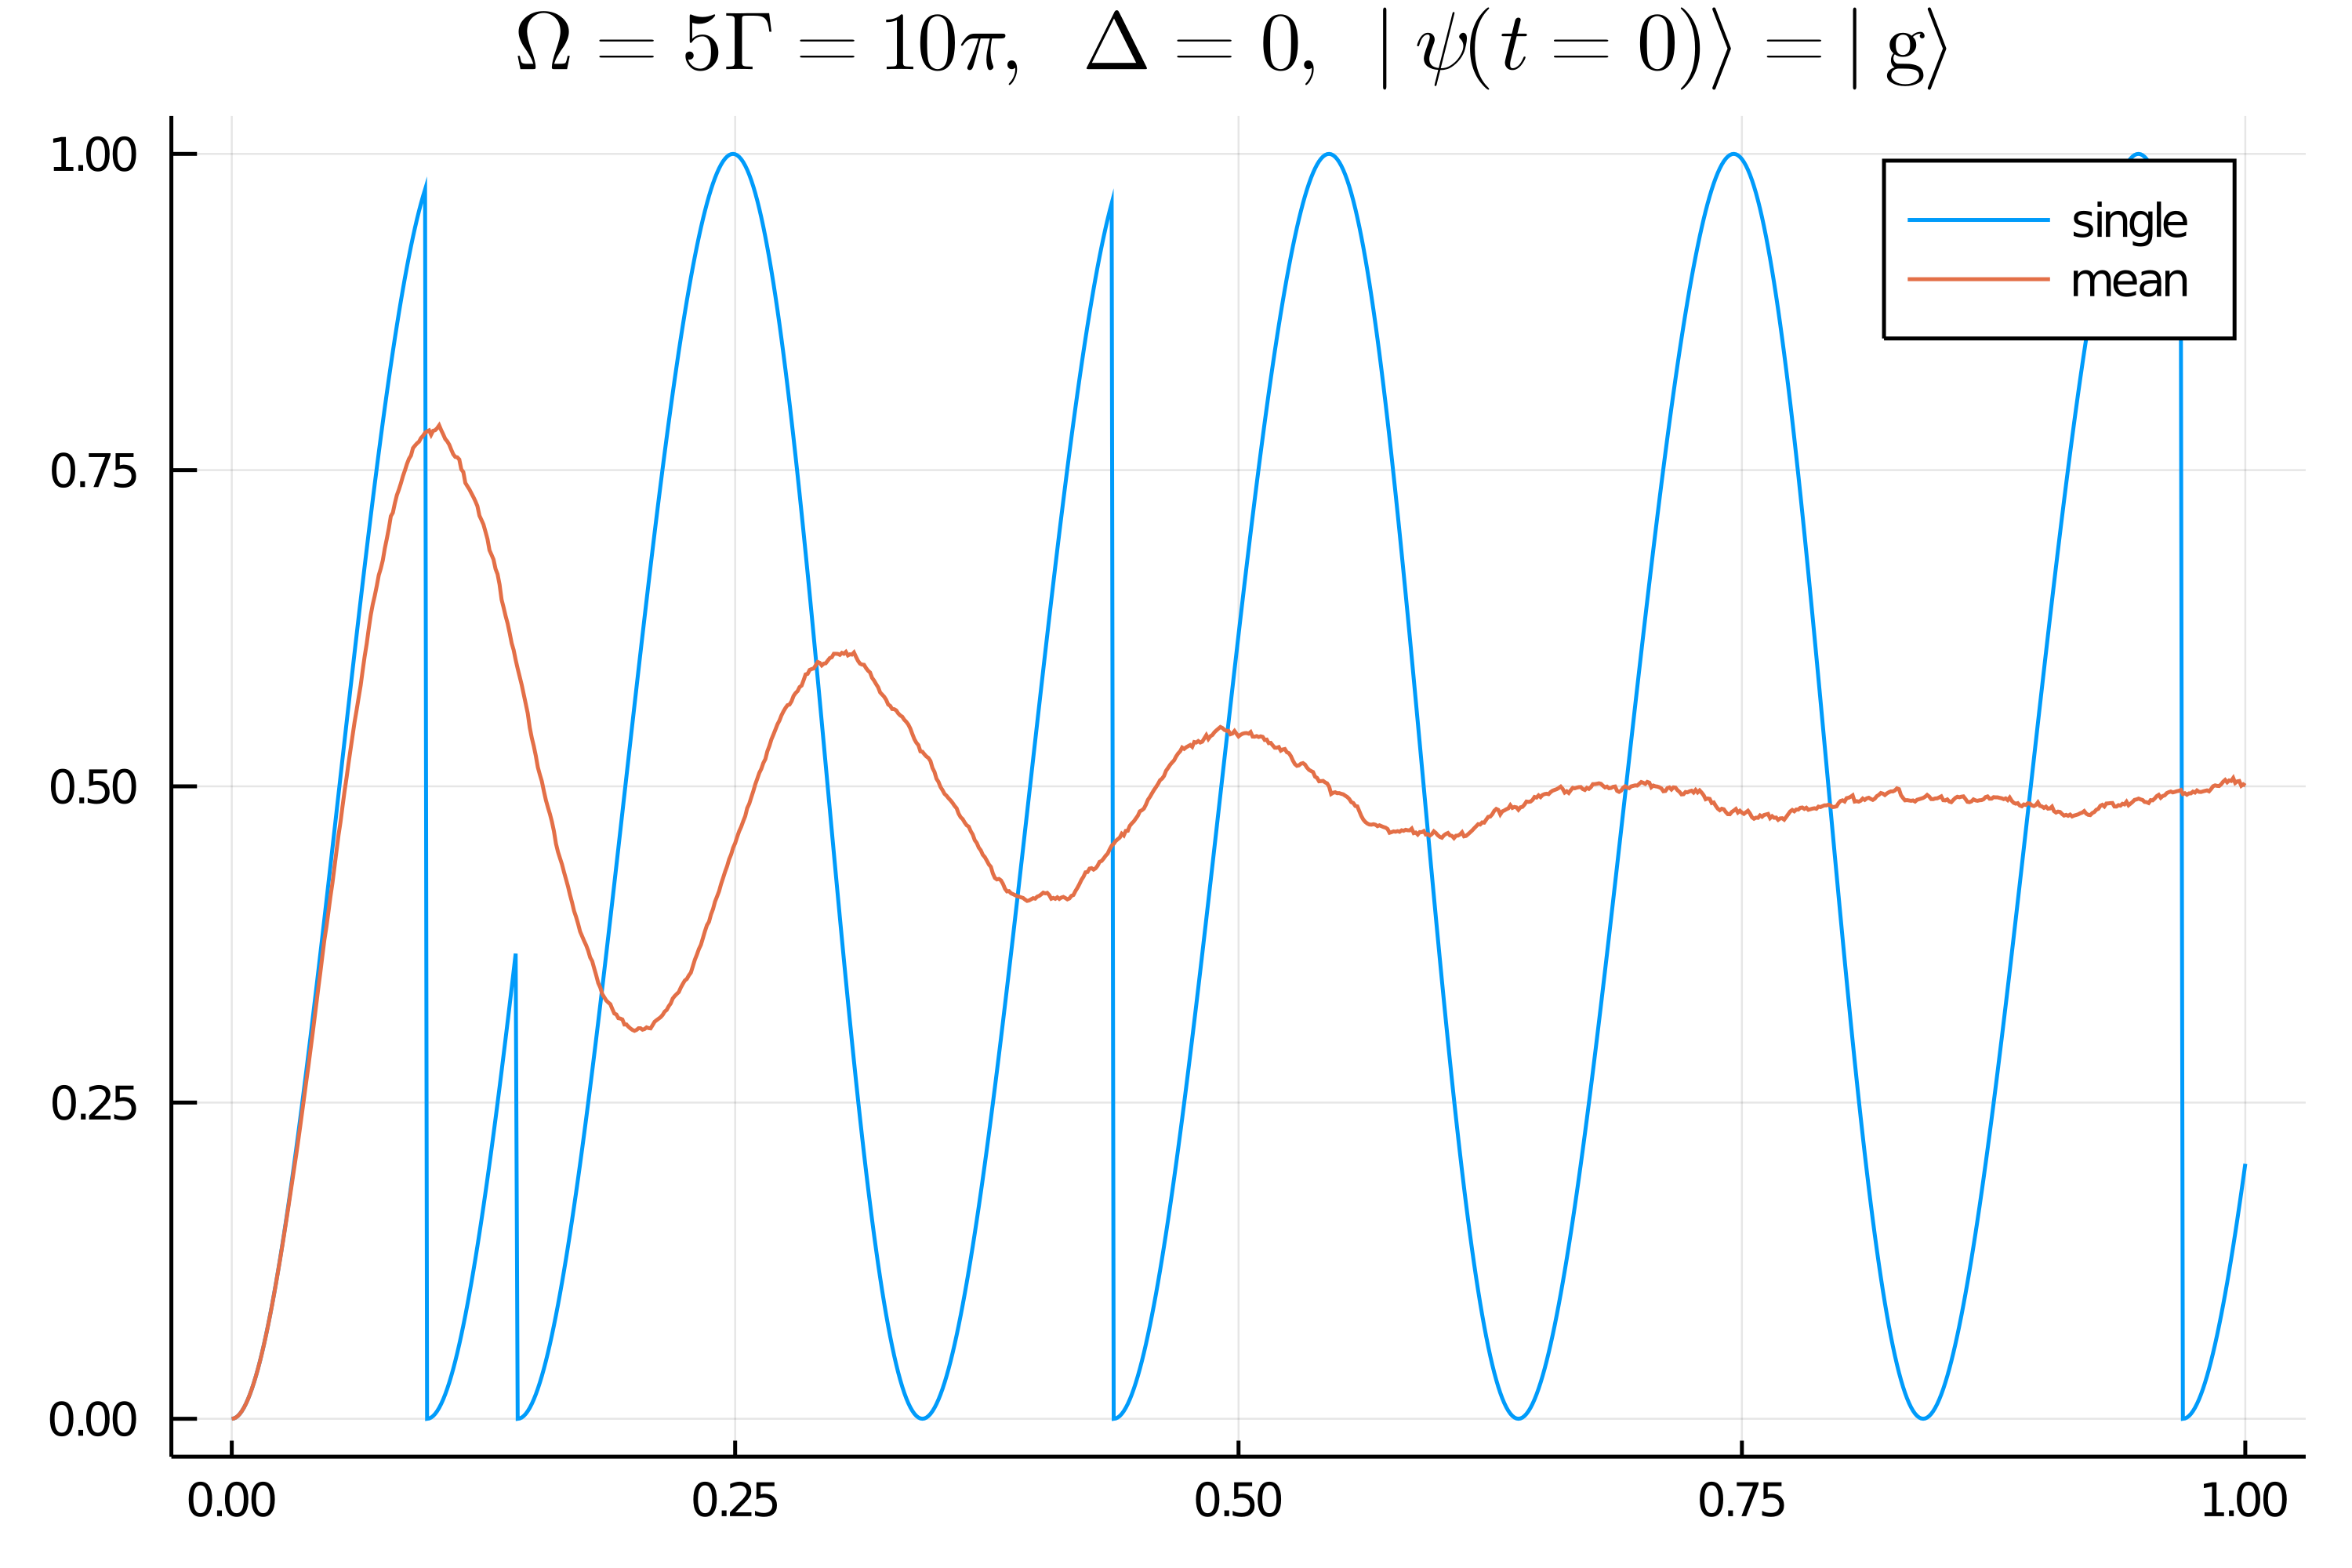
\includegraphics[width=\textwidth]{rwf-1.png}
        \subcaption{}
    \end{subfigure}
    \begin{subfigure}{0.45\textwidth}
        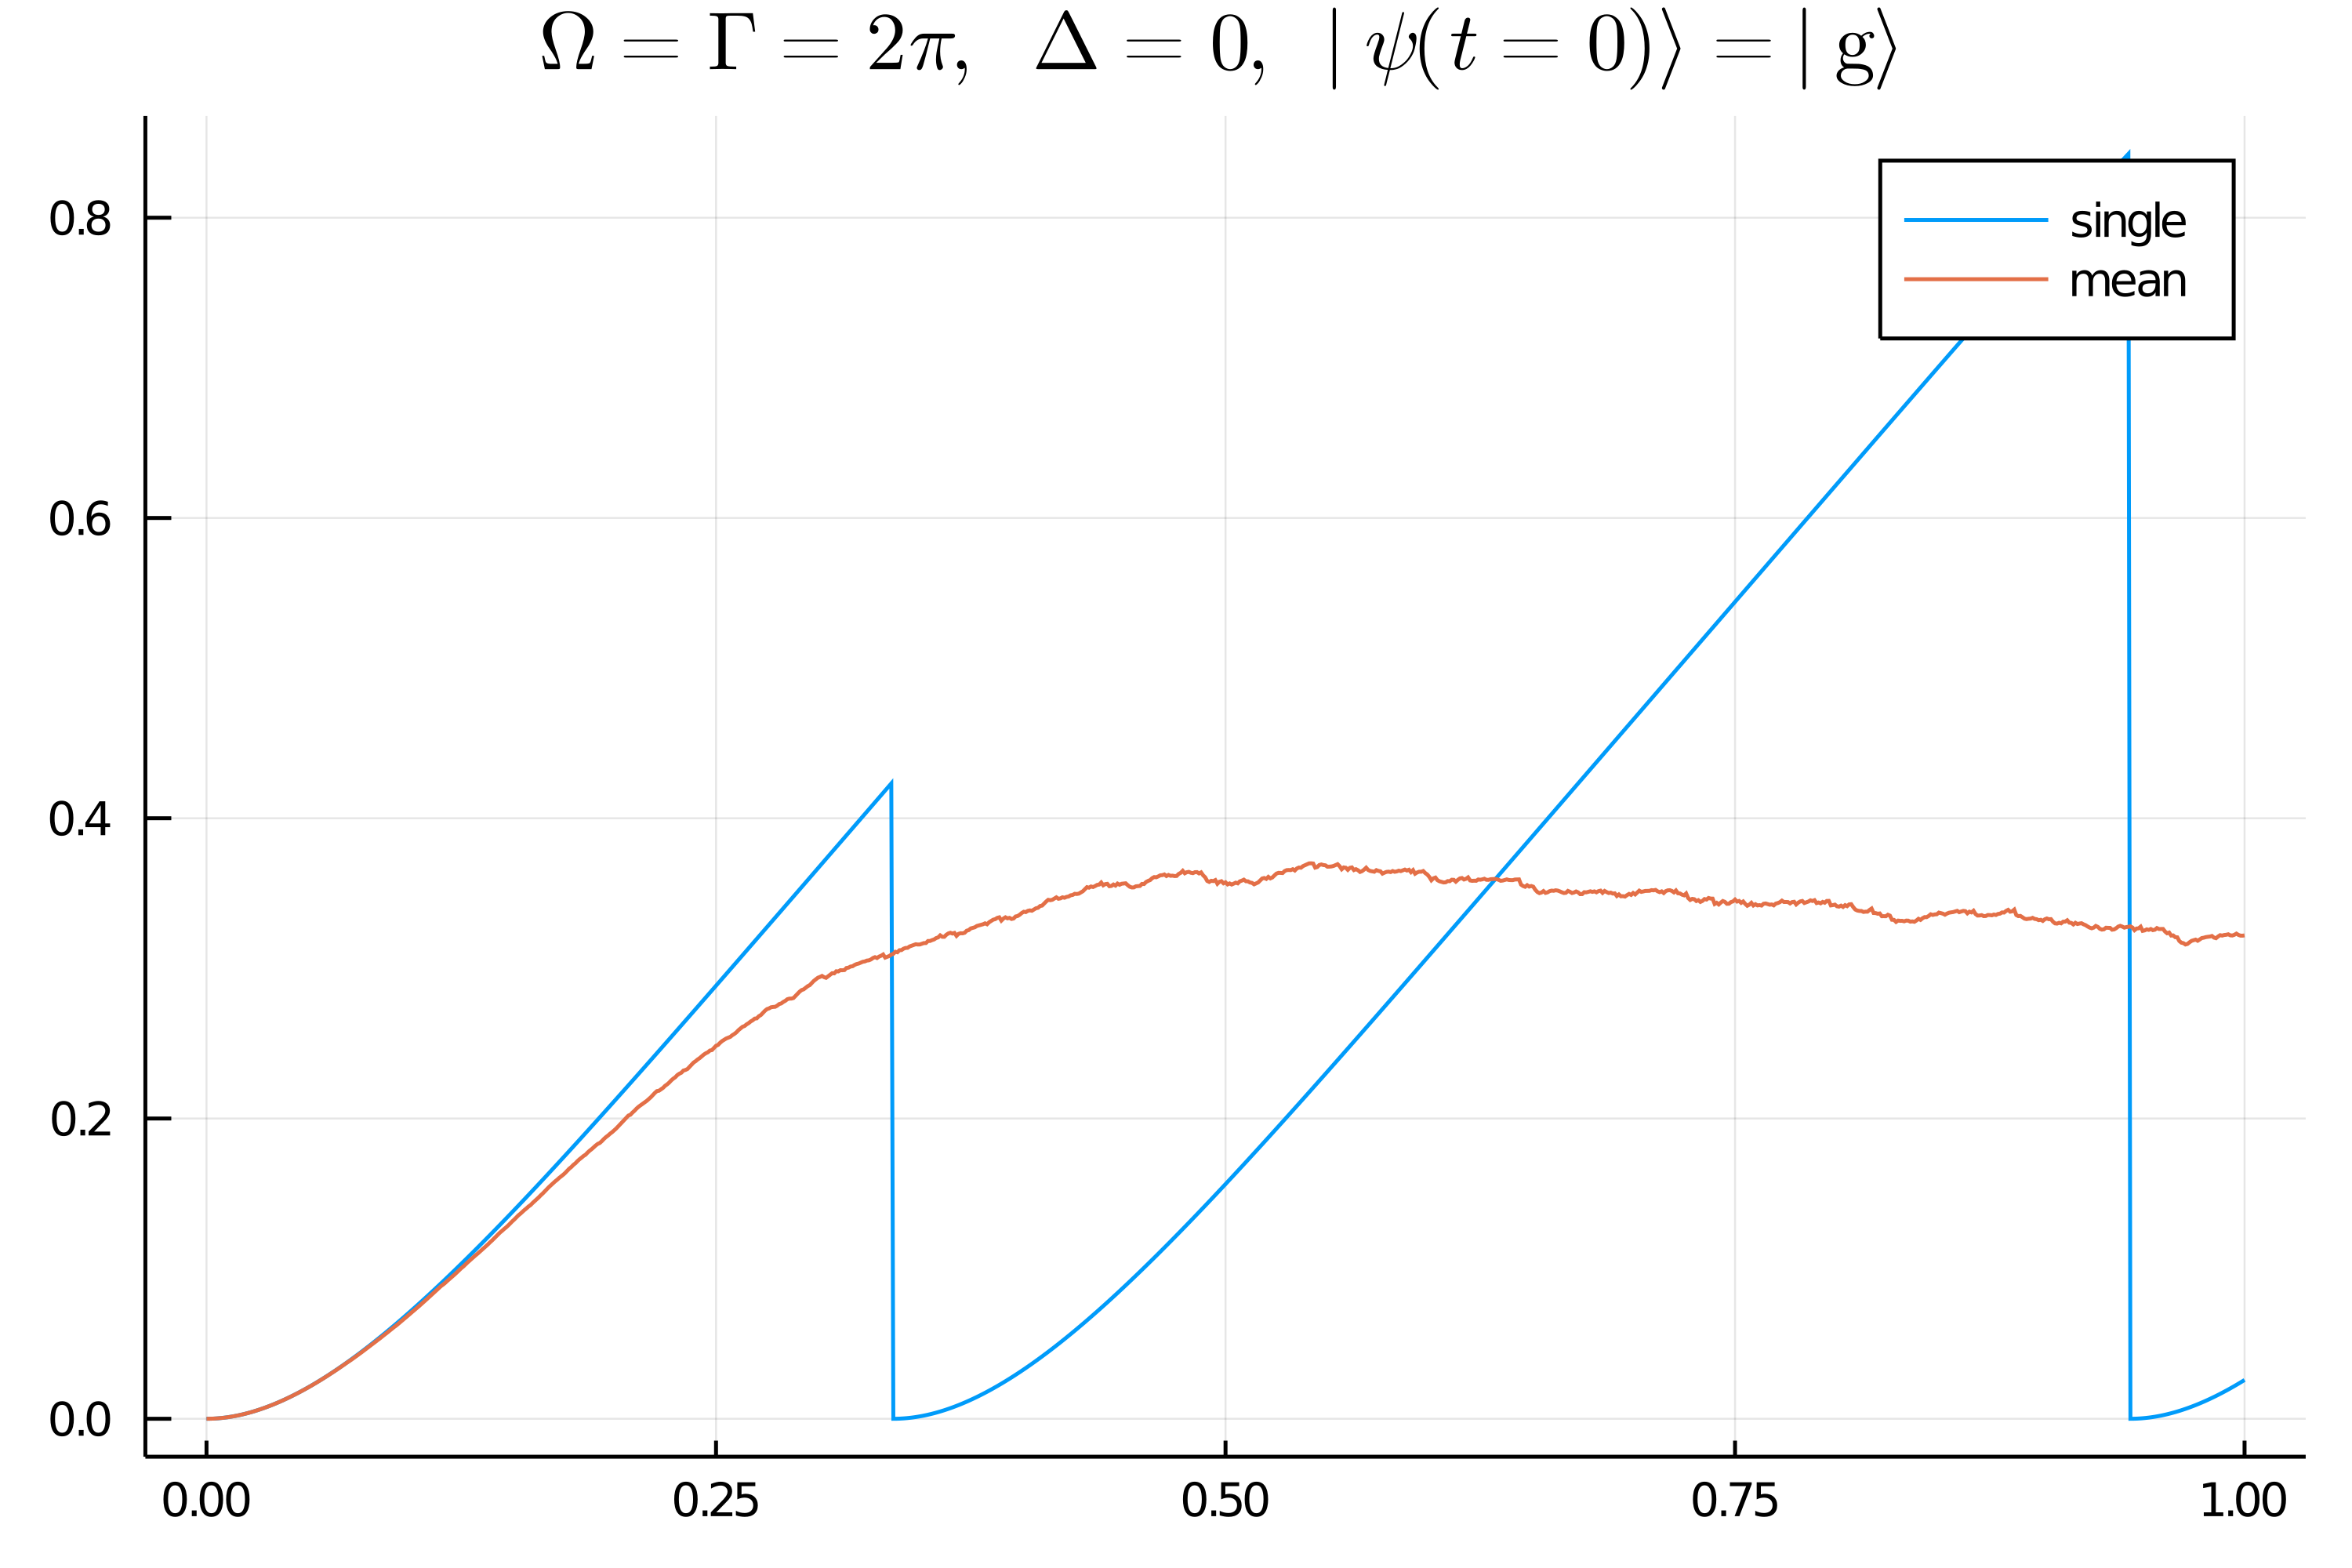
\includegraphics[width=\textwidth]{rwf-2.png}
        \subcaption{}
    \end{subfigure}
    \begin{subfigure}{0.45\textwidth}
        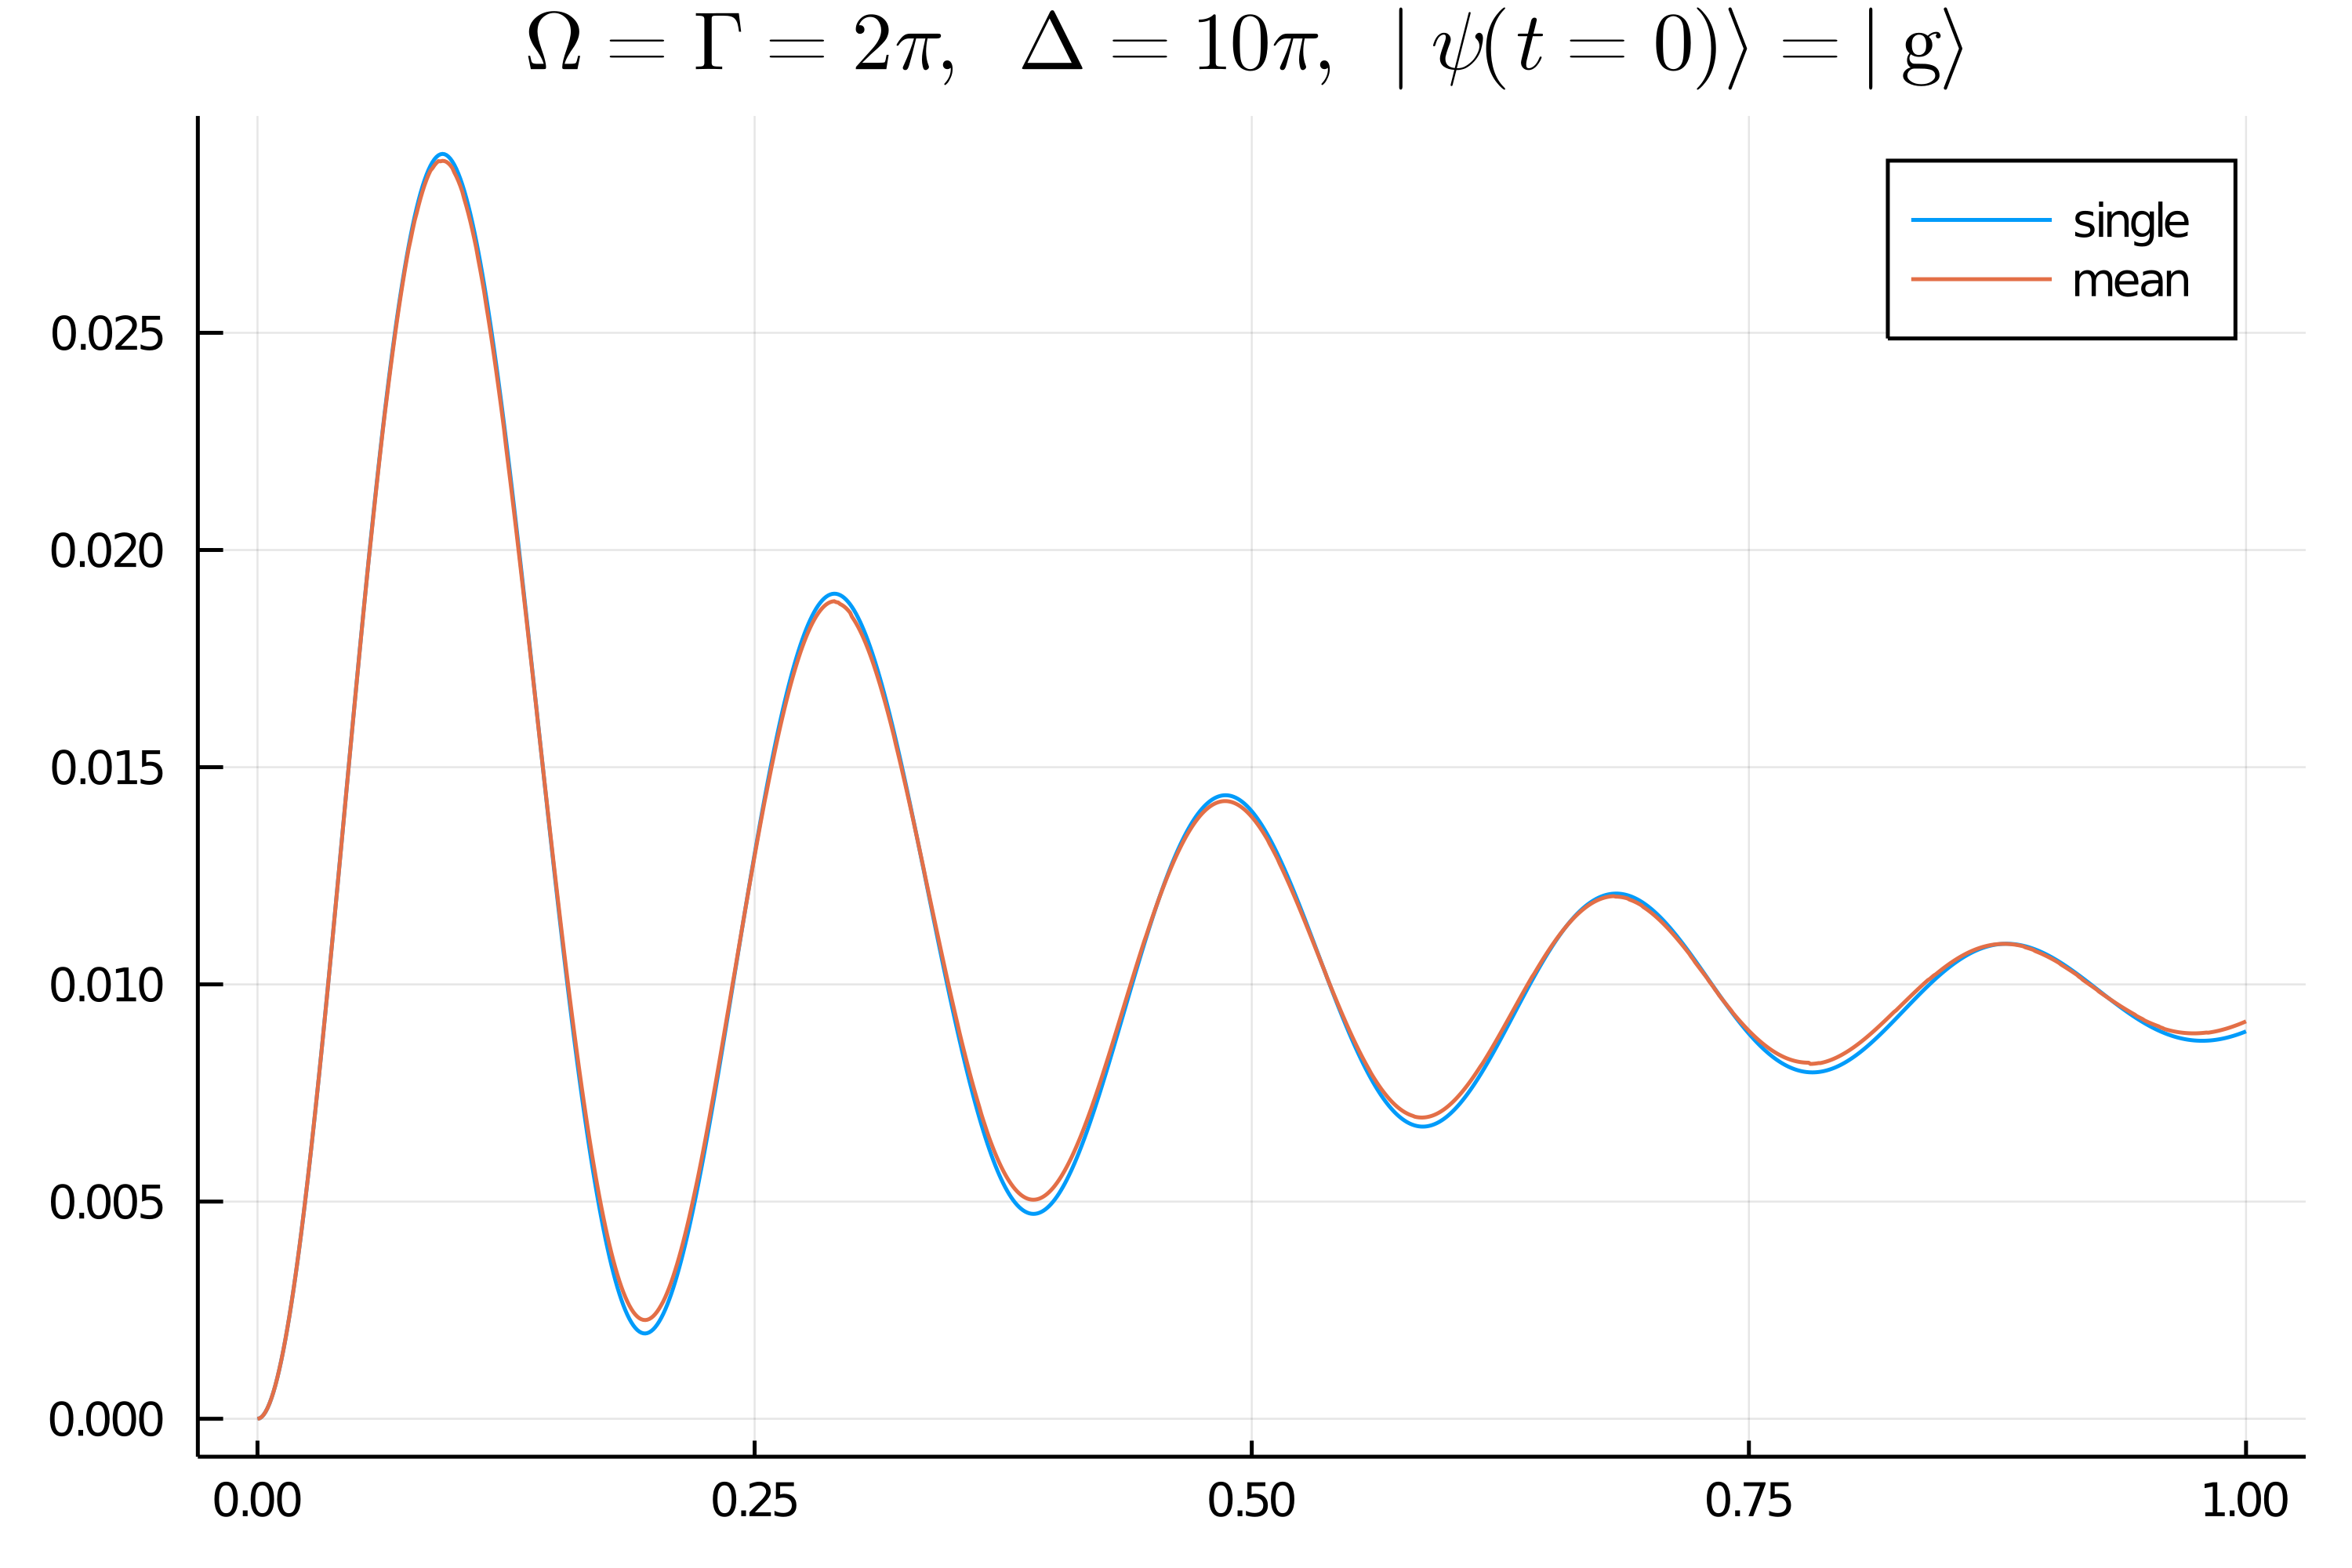
\includegraphics[width=\textwidth]{rwf-3.png}
        \subcaption{}
    \end{subfigure}
    \begin{subfigure}{0.45\textwidth}
        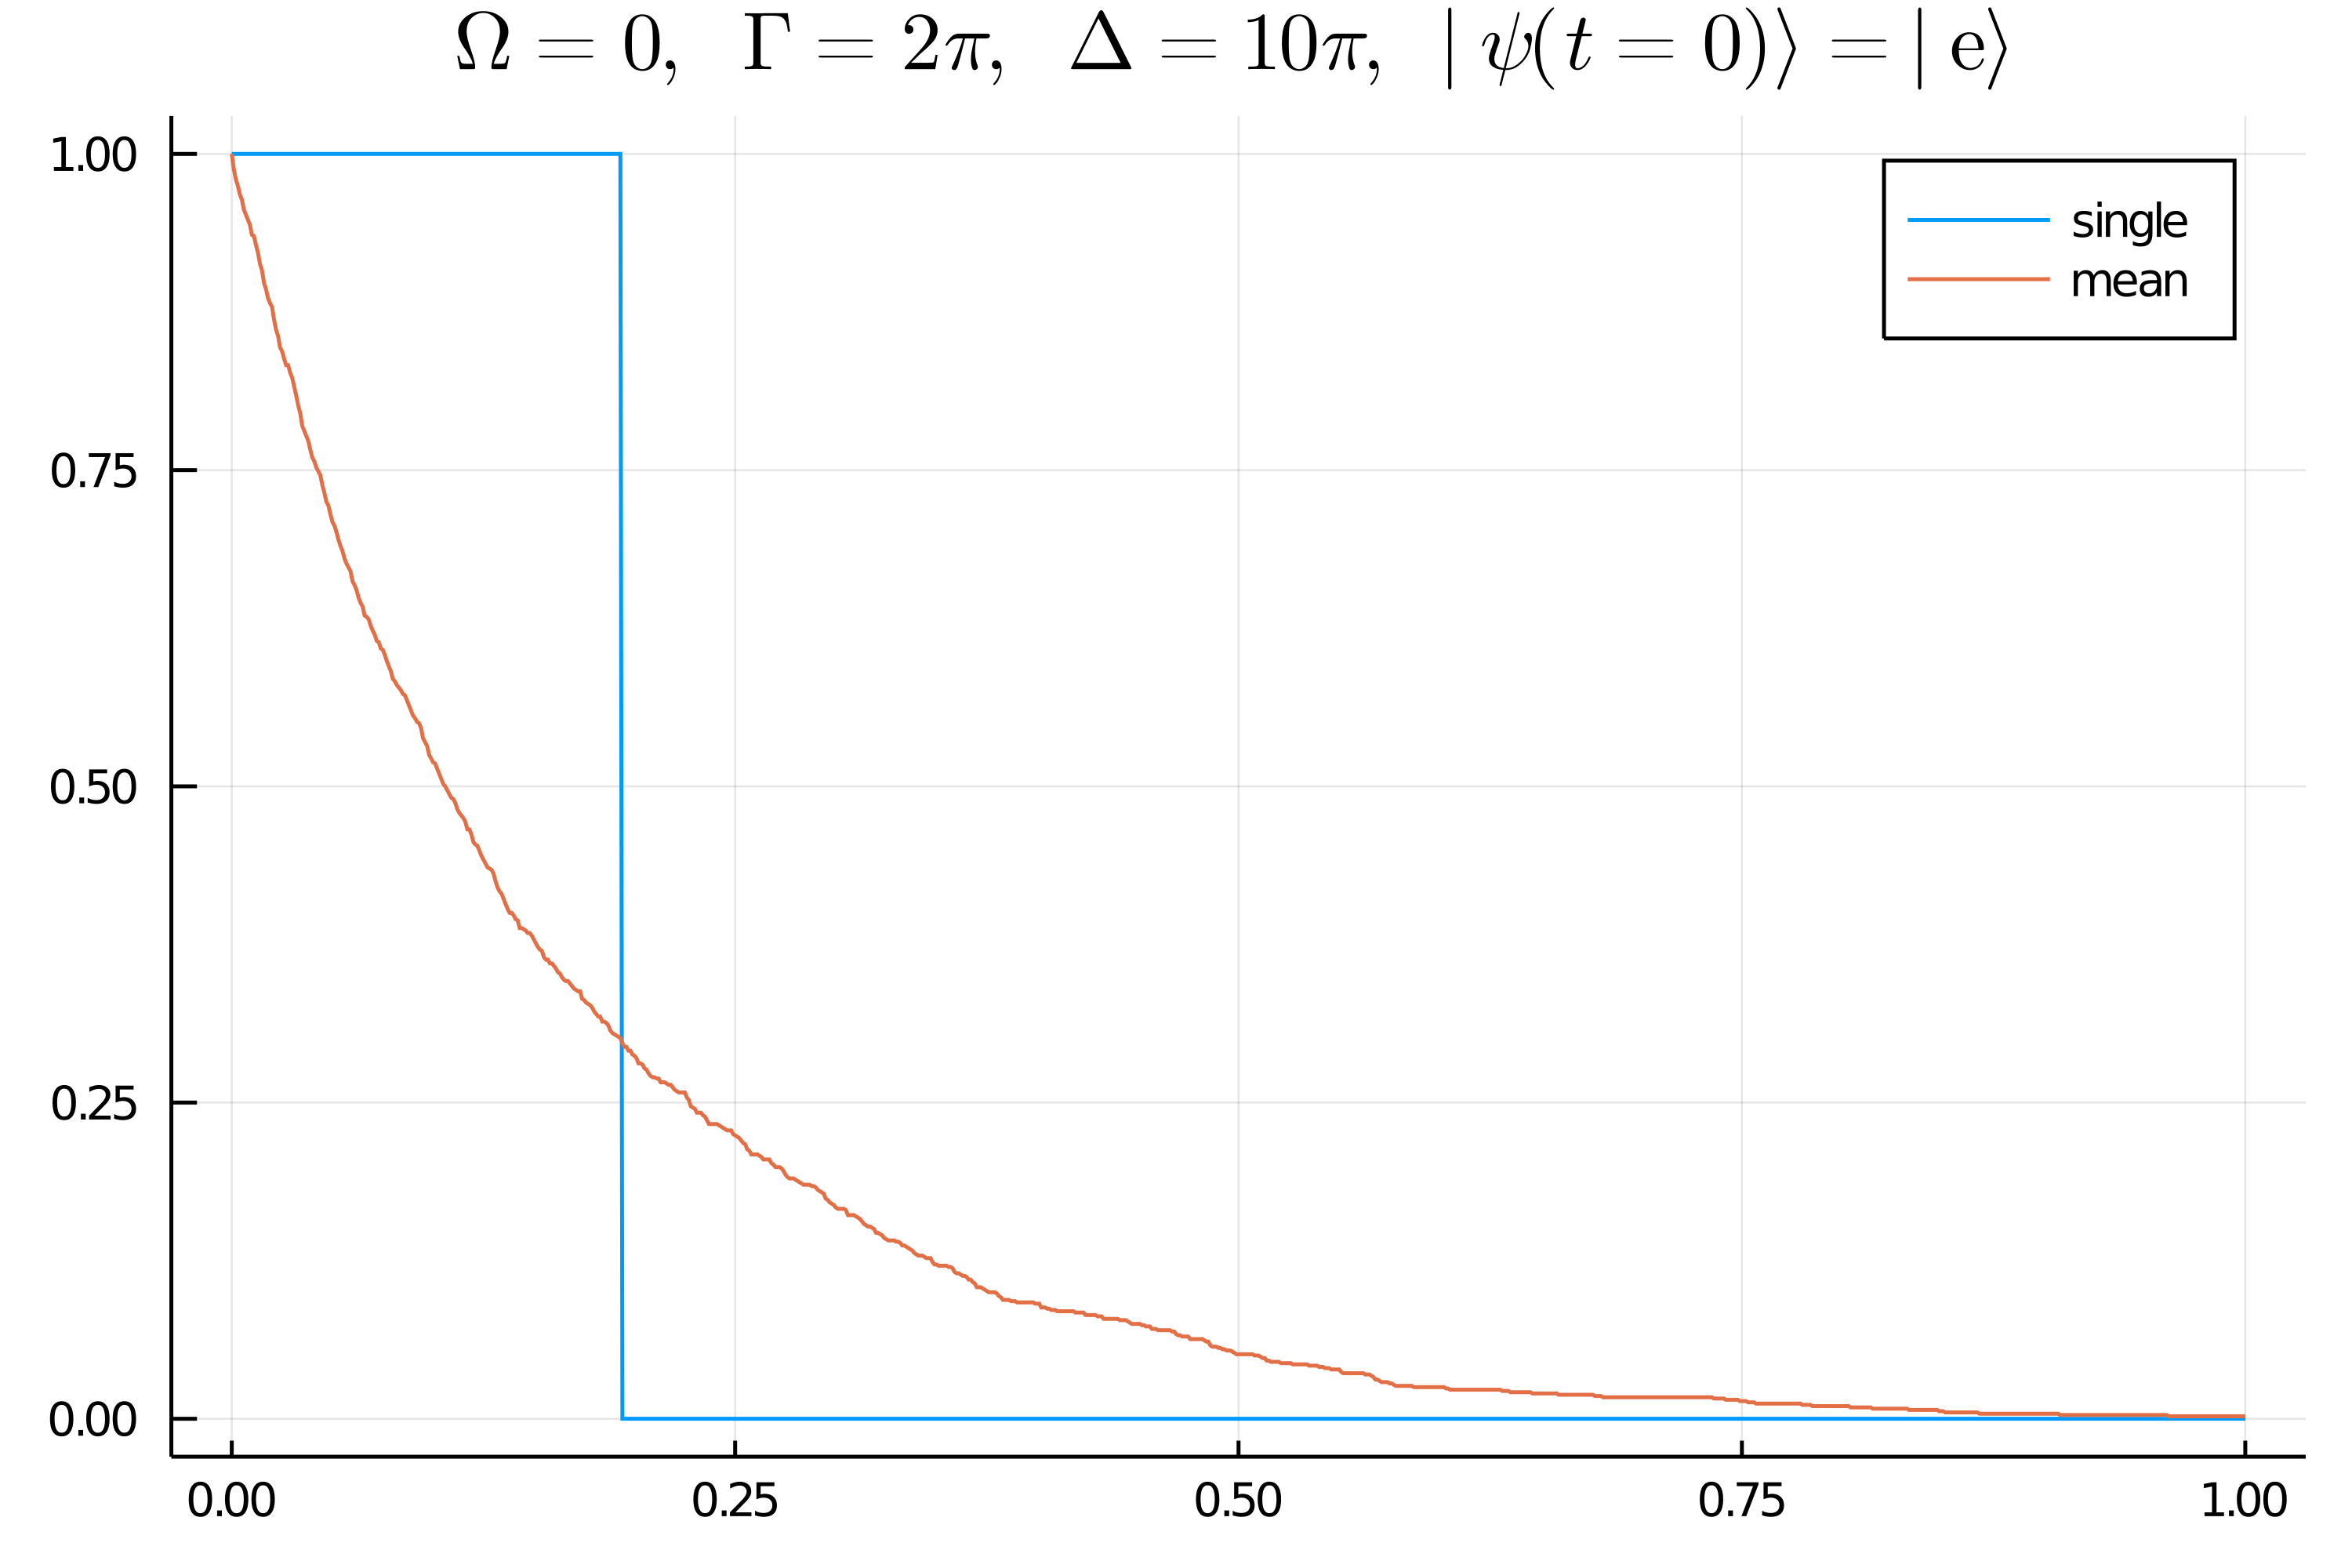
\includegraphics[width=\textwidth]{rwf-4.png}
        \subcaption{}
    \end{subfigure}
    \begin{subfigure}{0.45\textwidth}
        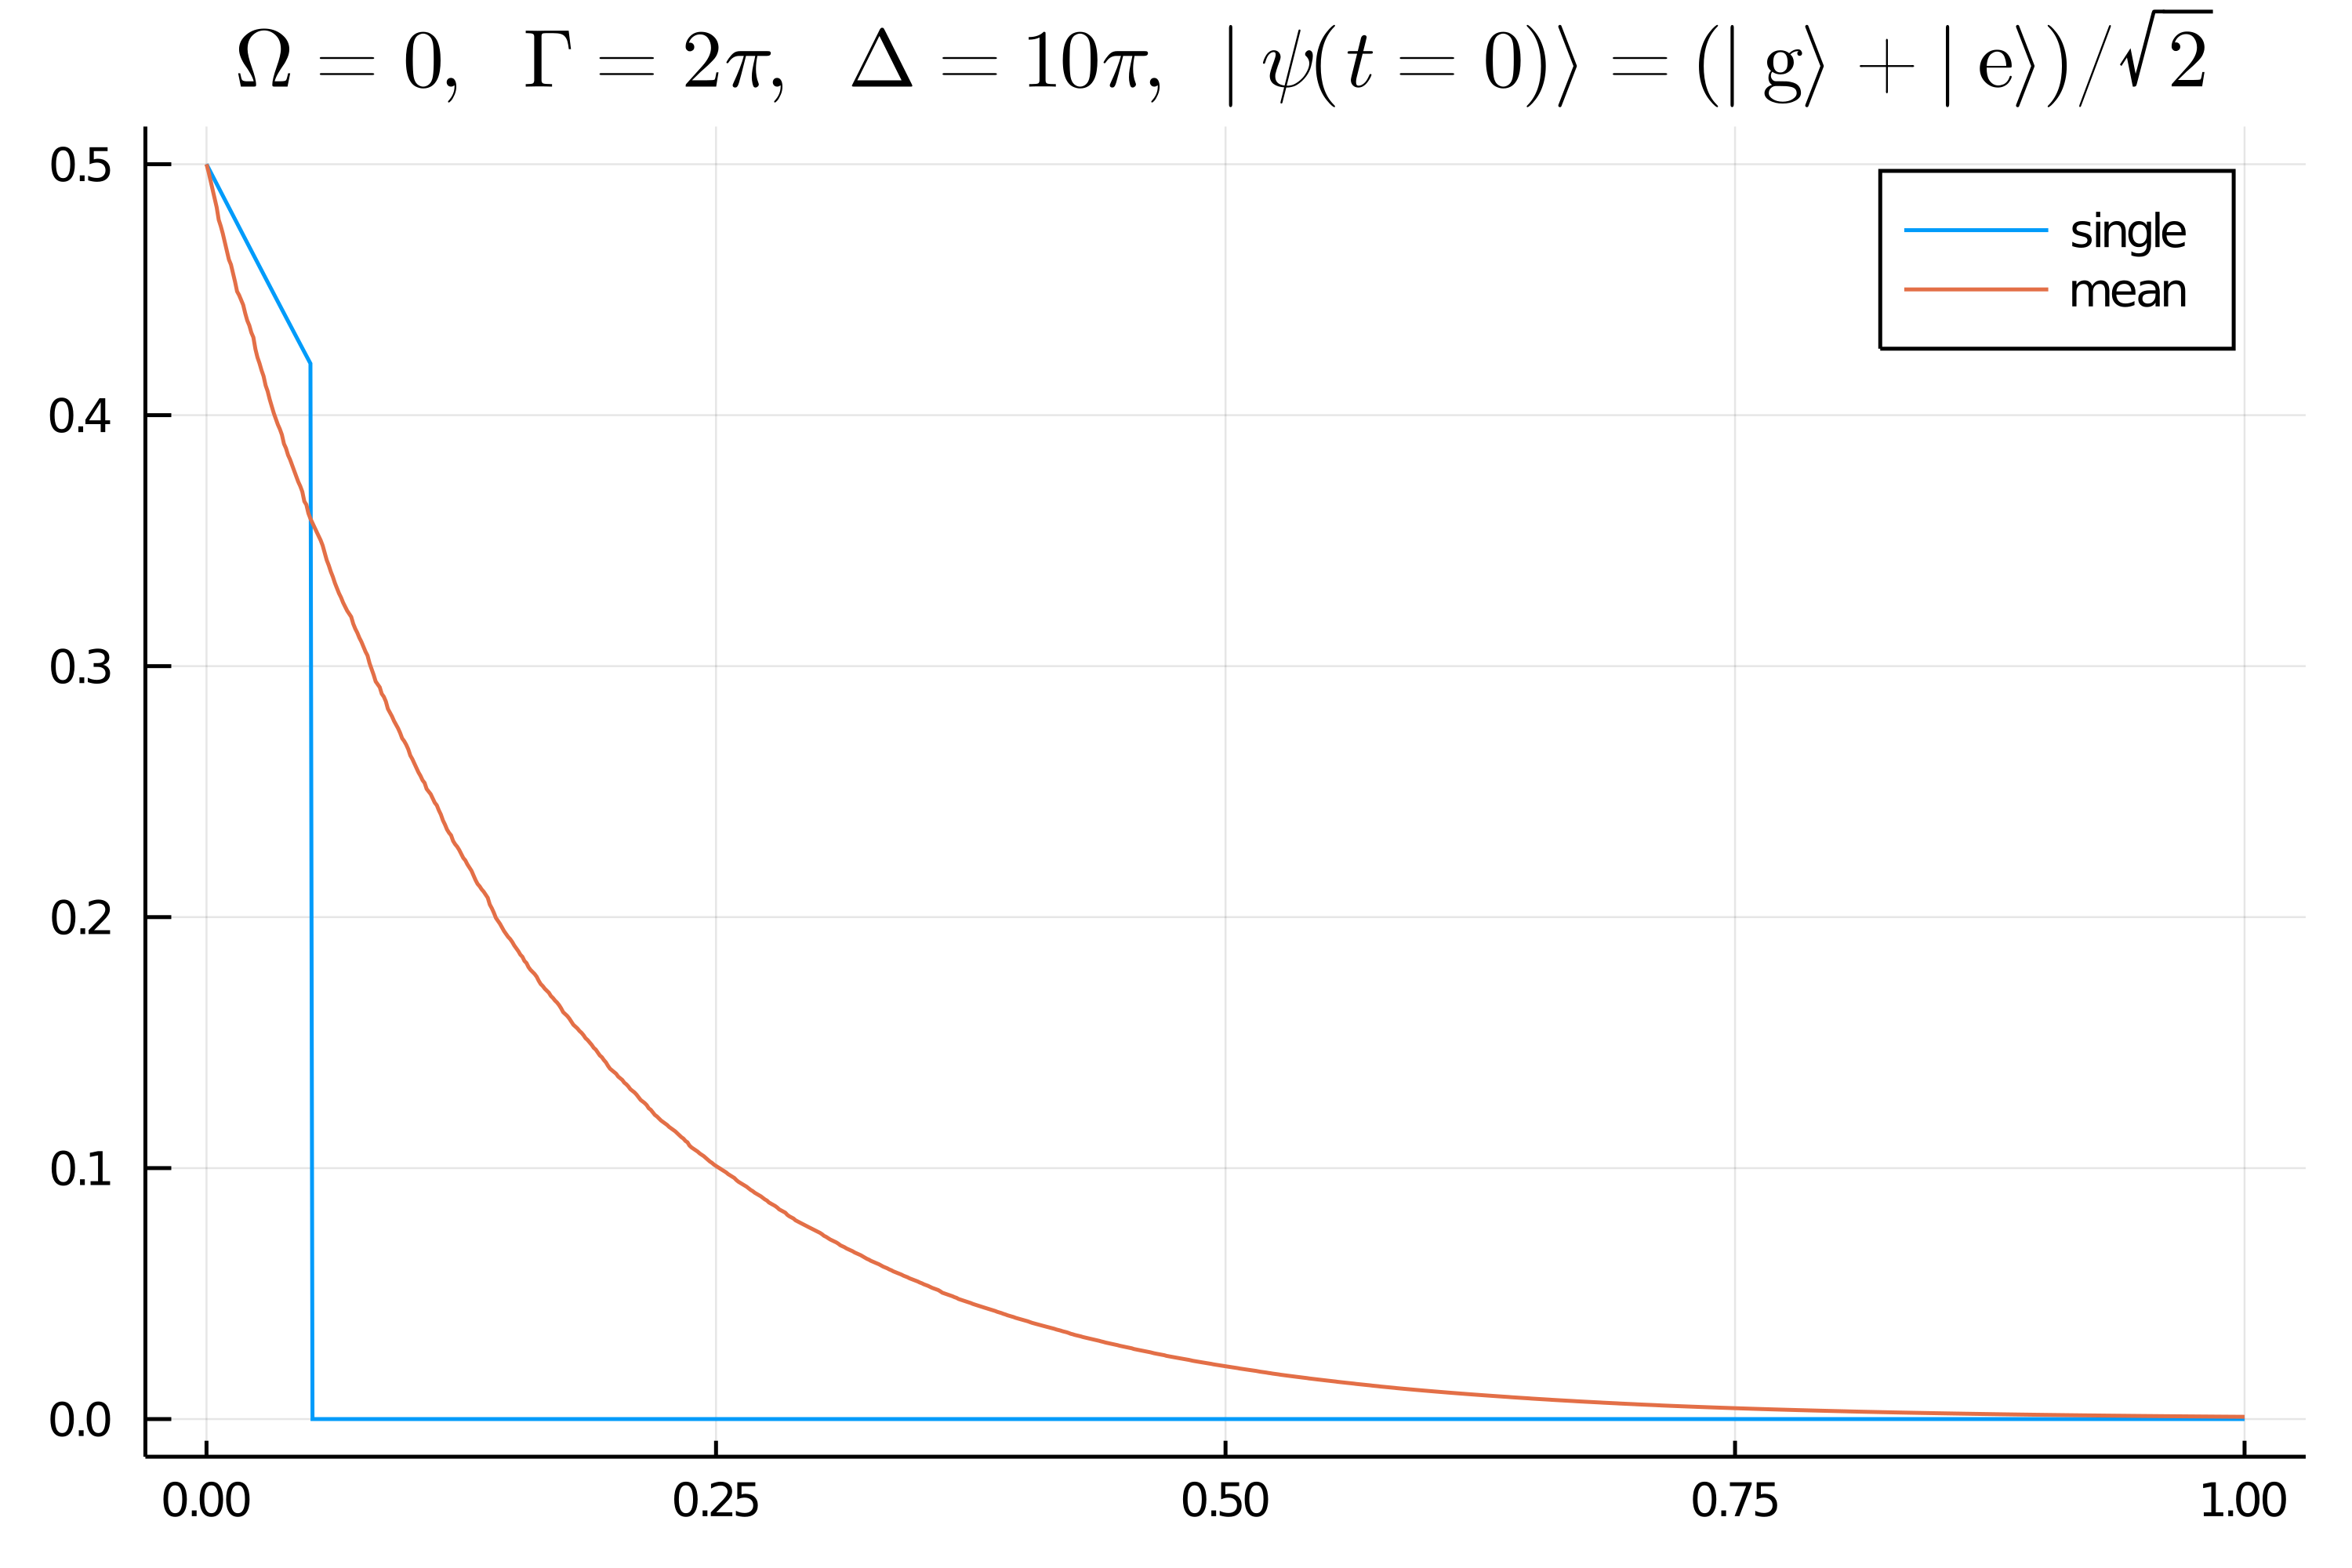
\includegraphics[width=\textwidth]{rwf-5.png}
        \subcaption{}
    \end{subfigure}
    \caption{Numerical simulated $P_\text{e}$.}
    \label{fig:numerical-wave}
\end{figure}

\paragraph{Solution} The code can be found \href{simulation.jl}{with this document}. The results are 
\prettyref{fig:numerical-wave}. The ``mean'' curves are the average value of 1000 runs. 

\paragraph{Discussion} The code in \href{simulation.jl}{with this document} has almost nothing more than
numerical solution of the Schrödinger equation. What we should note is that the numerical format 
\begin{equation}
    \ket*{\psi(t + \Delta t)} = \left( 1 - \frac{1}{\ii \hbar} H_\text{eff} \Delta t \right) \ket*{\psi(t)}
\end{equation}
may not be stable, and to make sure the error is acceptable, we need to use a very small $\Delta t$.

Calculating a figure in \prettyref{fig:numerical-wave} takes about 30 seconds on my computer. Considering 
an atom in an external optical field where spontaneous radiation is important is actually a quite complex
system, we should say the random wave function method is shockingly fast. The reason why it is fast is because 
we manage to not calculate the (often large) density matrix directly, but encode its classical fluctuation 
into different random wave function trajectories.

\paragraph{}

\begin{figure}
    \centering
    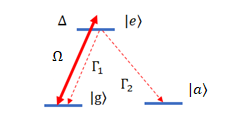
\includegraphics[width=0.4\textwidth]{fig1.png}
    \caption{A three-level $\Lambda$ system}
    \label{fig:sys-1}
\end{figure}

\paragraph{Stochastic wave function of a $\Lambda$ system} \prettyref{fig:sys-1} is a three-level $\Lambda$ system.
(a) Write down the effective Hamiltonian and quantum jump operators for \prettyref{fig:sys-1}.
(b) Suppose $\ket*{\psi_\text{s}(t=0)} = \ket*{\text{g}}$. Describe how the wave function evolves using pseudocode.
(c) Consider a case in which there is no quantum jump in $0 < t < t_0$. Find the time evolution of the 
wave function and the scattering rate 
\begin{equation}
    \gamma_1 = \expval*{C_1^\dagger C_1}{\psi_\text{s}}, \quad \gamma_2 = \expval*{C_2^\dagger C_2}{\psi_\text{s}}.
\end{equation}
(d) Plot the time evolution of $\gamma_1$ and $\gamma_2$ under the circumstance of
(i) $\Delta = 0, \Omega \gg \Gamma_1 \gg \Gamma_2$;
(ii) $\Omega = 2 \Delta \gg \Gamma_1 \gg \Gamma_2$;
(iii) $\Delta = 0, \Omega \ll \Gamma_1 , \Gamma_2$.

\paragraph{Solution} \begin{itemize}
\item[(a)] The effective Hamiltonian is
\begin{equation}  
    \begin{aligned}
        H_\text{eff} &= - \hbar \Delta \dyad{\text{e}} + \left( \frac{1}{2} \hbar \Omega \dyad{\text{e}}{\text{g}} + \text{h.c.} \right) - \frac{\ii \hbar}{2} (C_1^\dagger C_1 + C_2^\dagger C_2) \\
        &= - \hbar (\Delta + \ii \Gamma / 2) \dyad{\text{e}} + \hbar (\Omega \dyad{\text{e}}{\text{g}} + \text{h.c.}) / 2,
    \end{aligned}
    \label{eq:h-eff-1}
\end{equation}  
where the quantum jump operators are 
\begin{equation}
    C_1 = \sqrt{\Gamma_1} \dyad*{\text{a}}{\text{e}}, \quad C_2 = \sqrt{\Gamma_2} \dyad*{\text{g}}{\text{e}},
\end{equation}
and 
\begin{equation}
    \Gamma = \Gamma_1 + \Gamma_2.
\end{equation}

\item[(b)] The time evolution can be described using the following algorithm.
 
\begin{algorithm*}[H]

    \DontPrintSemicolon
    \SetAlgoLined

    \SetKwInOut{Input}{input}
    \SetKwInOut{Output}{output}
    \Input{Time step $\Delta t$, maximal time $t_0$}

    Initialize an array $\{ \ket*{\psi_\text{s}(t)} \}_{t=n \Delta t}$ of wave functions with $t_0 / \Delta t$ elements  \;
    \For{$t \in 0 : \Delta t : t_0$}{
        Pick up a uniformly distributed random number $x$ between $0$ and $1$ \;
        $P_\text{g} \leftarrow \Delta t \expval*{C_1^\dagger C_1}{\psi_\text{s}(t)}$ \;
        $P_\text{a} \leftarrow \Delta t \expval*{C_2^\dagger C_2}{\psi_\text{s}(t)}$ \;
        \tcp*[h]{jumping to $\ket*{\text{g}}$} \;
        \uIf{
            $0 < x < P_\text{g}$}{
            $\ket*{\psi_\text{s}(t + \Delta t)} \leftarrow \text{normalized } C_1 \ket*{\psi_\text{s}(t)} $ \;
        }
        \tcp*[h]{jumping to $\ket*{\text{a}}$} \;
        \uElseIf{
            $P_\text{g} < x < P_\text{g} + P_\text{a}$
        }{
            $\ket*{\psi_\text{s}(t + \Delta t)} \leftarrow \text{normalized } C_2 \ket*{\psi_\text{s}(t)} $ \;
        }
        \tcp*[h]{evolution according to the effective Hamiltonian} \;
        \Else{
            $\ket*{\psi_\text{s}(t + \Delta t)} \leftarrow \text{normalized } \ket*{\psi_\text{s}(t)} + \frac{\Delta t}{\ii \hbar} H_\text{eff} \ket*{\psi_\text{s}(t)} $ \;
        }
    }
    
  \end{algorithm*}
\item[(c)] The wave function in this case evolves purely according to $H_\text{eff}$. Since Schrödinger equation
is linear, we can leave the normalization to the end of our calculation. Note that \eqref{eq:h-eff-1} actually
does not contain $\ket*{\text{a}}$ explicitly, nor does the initial state $\ket*{\text{g}}$. Therefore we can 
work in the two-level system spanned by $\ket*{\text{e}}$ and $\ket*{\text{g}}$. The effective Hamiltonian is 
\begin{equation}
    H_\text{eff} = \hbar \pmqty{0 & \Omega^* / 2 \\ \Omega / 2 & - (\Delta + \ii \Gamma / 2)},
\end{equation}
where we let $\ket*{\text{g}}$ be the first component and $\ket*{\text{e}}$ the second. We have the decomposition 
\begin{equation}
    H_\text{eff} = - \frac{\hbar}{2} (\Delta + \ii \Gamma) + \frac{\hbar}{2} \vb*{\Omega} \cdot \vb*{\sigma}, \quad 
    \vb*{\Omega} = (\Omega_\text{r}, \Omega_\text{i}, \Delta + \ii \Gamma / 2).
    \label{eq:h-eff-1-decomp}
\end{equation}
Note here we cannot ``shift the energy zero point'' to reshape the Hamiltonian into $\vb*{\Omega} \cdot \vb*{\sigma}$, because 
the value damping rate has physical meaning. Applying \eqref{eq:h-eff-1-decomp} on $\ket*{\text{g}}$, we have 
\[
    \begin{aligned}
        \ee^{- \ii H_\text{eff} t / \hbar} \ket*{\text{g}} &= 
        \ee^{\ii t (\Delta + \ii \Gamma / 2) / 2} \ee^{- \ii t \vb*{\Omega} \cdot \vb*{\sigma} / 2} \ket*{\text{g}} \\
        &= \ee^{- \Gamma t / 4} \ee^{\ii \Delta t / 2} \left( \sigma^0 \cos \frac{\abs*{\vb*{\Omega}} t}{2}  
        - \frac{\ii \vb*{\Omega} \cdot \vb*{\sigma}}{\abs*{\vb*{\Omega}}} \sin \frac{\abs*{\vb*{\Omega}} t}{2} \right) \ket*{\text{g}} \\
        &= \ee^{- \Gamma t / 4} \ee^{\ii \Delta t / 2} \left(\cos \frac{\abs*{\vb*{\Omega}} t}{2} \ket*{\text{g}} - \left( \frac{\Omega_\text{r}}{\abs*{\vb*{\Omega}}} \ket*{\text{e}} + \frac{\ii \Omega_\text{i}}{\abs*{\vb*{\Omega}}} \ket*{\text{e}} + \frac{\Delta + \ii \Gamma / 2}{\abs*{\vb*{\Omega}}} \ket*{\text{g}} \right) \ii \sin \frac{\abs*{\vb*{\Omega}} t}{2} \right)  ,
    \end{aligned}
\] 
where 
\begin{equation}
    \abs*{\vb*{\Omega}} = \sqrt{\abs*{\Omega}^2 + \Delta^2 - \Gamma^2 / 4 + \ii \Delta \Gamma}.
    \label{eq:omega-abs-2}
\end{equation}
\begin{note*}{}{}
    Note that here $\abs*{\vb*{n}}$ is defined as $\sqrt{\vb*{n}^\top \vb*{n}}$ instead of 
    $\sqrt{\vb*{n}^\dagger \vb*{n}}$, because to make 
    \[
        \ee^{\ii \alpha \vb*{n} \cdot \vb*{\sigma}} = \sigma^0 \cos \alpha + \ii \vb*{n} \cdot \vb*{\sigma} \sin \alpha
    \]
    hold, it is required that 
    \[
        (\vb*{n} \cdot \vb*{\sigma})^2 = \sigma^0,
    \]
    which is equivalent to $\vb*{n} \cdot \vb*{n} = 1$, considering $\acomm*{\sigma^i}{\sigma^j} = 0$ 
    when $i \neq j$. What is important here, therefore, is $\vb*{n} \cdot \vb*{n}$.
\end{note*}
Therefore we have (we have omitted the complex factors, since they will be canceled by normalization anyway) 
\begin{equation}
    \ket*{\psi_\text{s}(t)} = \frac{1}{C} \left( \cos \frac{\abs*{\vb*{\Omega}} t}{2} - \ii \frac{\Delta + \ii \Gamma / 2}{\abs*{\vb*{\Omega}}} \sin \frac{\abs*{\vb*{\Omega}} t}{2}  \right) \ket*{\text{g}} - \frac{\ii \Omega}{\abs*{\vb*{\Omega}}} \sin \frac{\abs*{\vb*{\Omega}} t}{2} \ket*{\text{e}},
\end{equation}
the normalization constant being 
\begin{equation}
    C = \sqrt{ \abs{\cos \frac{\abs*{\vb*{\Omega}} t}{2} - \ii \frac{\Delta + \ii \Gamma / 2}{\abs*{\vb*{\Omega}}} \sin \frac{\abs*{\vb*{\Omega}} t}{2} }^2 + \frac{\abs{\Omega}^2}{\abs*{\vb*{\Omega}}^2} \sin^2 \frac{\abs*{\vb*{\Omega}} t}{2} }.
\end{equation}
Since  
\[
    C_1^\dagger C_1 = \Gamma_1 \dyad{\text{e}}, \quad C_2^\dagger C_2 = \Gamma_2 \dyad{\text{e}},
\]
it is then straightforward that 
\begin{equation}
    \gamma_1 = \frac{\Gamma_1}{{C}^2} \frac{\Omega^2}{\abs*{\vb*{\Omega}}^2} \abs{\sin \frac{\abs*{\vb*{\Omega}} t}{2}}^2,
    \quad \gamma_2 = \frac{\Gamma_2}{{C}^2} \frac{\Omega^2}{\abs*{\vb*{\Omega}}^2} \abs{\sin \frac{\abs*{\vb*{\Omega}} t}{2}}^2.
\end{equation}
Note that in these equations $\abs{\vb*{\Omega}}^2$ means the norm, i.e. $\abs{\vb*{\Omega}} \cdot \abs*{\vb*{\Omega}}^*$. 

The scattering rates are calculated under the assumption that no quantum jump happened before, so what they mean
are actually the probabilities that ``no quantum jump happened before, and a quantum jump will happen in the next 
second''.

\begin{figure}
    \centering
    \begin{subfigure}{0.45\textwidth}
        \centering
        

\tikzset{every picture/.style={line width=0.75pt}} %set default line width to 0.75pt        

\begin{tikzpicture}[x=0.75pt,y=0.75pt,yscale=-0.7,xscale=0.7]
%uncomment if require: \path (0,300); %set diagram left start at 0, and has height of 300

%Straight Lines [id:da13890275119088025] 
\draw    (107,266) -- (433,266) ;
\draw [shift={(435,266)}, rotate = 180] [fill={rgb, 255:red, 0; green, 0; blue, 0 }  ][line width=0.08]  [draw opacity=0] (12,-3) -- (0,0) -- (12,3) -- cycle    ;
%Straight Lines [id:da045483371567715425] 
\draw    (107,266) -- (107,53.06) ;
\draw [shift={(107,51.06)}, rotate = 90] [fill={rgb, 255:red, 0; green, 0; blue, 0 }  ][line width=0.08]  [draw opacity=0] (12,-3) -- (0,0) -- (12,3) -- cycle    ;
%Shape: Wave [id:dp47457281322525113] 
\draw   (107,266) .. controls (111.52,266) and (115.42,246.75) .. (119.5,226.53) .. controls (123.58,206.31) and (127.48,187.06) .. (132,187.06) .. controls (136.52,187.06) and (140.42,206.31) .. (144.5,226.53) .. controls (148.58,246.75) and (152.48,266) .. (157,266) .. controls (161.52,266) and (165.42,246.75) .. (169.5,226.53) .. controls (173.58,206.31) and (177.48,187.06) .. (182,187.06) .. controls (186.52,187.06) and (190.42,206.31) .. (194.5,226.53) .. controls (198.58,246.75) and (202.48,266) .. (207,266) .. controls (211.52,266) and (215.42,246.75) .. (219.5,226.53) .. controls (223.58,206.31) and (227.48,187.06) .. (232,187.06) .. controls (236.52,187.06) and (240.42,206.31) .. (244.5,226.53) .. controls (248.58,246.75) and (252.48,266) .. (257,266) .. controls (261.52,266) and (265.42,246.75) .. (269.5,226.53) .. controls (273.58,206.31) and (277.48,187.06) .. (282,187.06) .. controls (286.52,187.06) and (290.42,206.31) .. (294.5,226.53) .. controls (298.58,246.75) and (302.48,266) .. (307,266) .. controls (311.52,266) and (315.42,246.75) .. (319.5,226.53) .. controls (323.58,206.31) and (327.48,187.06) .. (332,187.06) .. controls (334.85,187.06) and (337.45,194.69) .. (340,205.38) ;
%Straight Lines [id:da9947339757320526] 
\draw    (340,205) -- (340,266.23) ;
%Shape: Wave [id:dp14242618932253137] 
\draw   (340.17,265.5) .. controls (344.69,265.5) and (348.59,246.25) .. (352.67,226.03) .. controls (356.74,205.81) and (360.64,186.56) .. (365.17,186.56) .. controls (369.69,186.56) and (373.59,205.81) .. (377.67,226.03) .. controls (381.74,246.25) and (385.64,265.5) .. (390.17,265.5) .. controls (394.69,265.5) and (398.59,246.25) .. (402.67,226.03) .. controls (404.62,216.33) and (406.54,206.85) .. (408.5,199.62) ;
%Straight Lines [id:da5738702488575167] 
\draw  [dash pattern={on 4.5pt off 4.5pt}]  (157,111.4) -- (157,265.4) ;
%Straight Lines [id:da6882547868056692] 
\draw    (109,144.4) -- (155,144.4) ;
\draw [shift={(157,144.4)}, rotate = 180] [fill={rgb, 255:red, 0; green, 0; blue, 0 }  ][line width=0.08]  [draw opacity=0] (12,-3) -- (0,0) -- (12,3) -- cycle    ;
\draw [shift={(107,144.4)}, rotate = 0] [fill={rgb, 255:red, 0; green, 0; blue, 0 }  ][line width=0.08]  [draw opacity=0] (12,-3) -- (0,0) -- (12,3) -- cycle    ;
%Straight Lines [id:da29886051300608063] 
\draw    (377,131.4) -- (346.89,191.61) ;
\draw [shift={(346,193.4)}, rotate = 296.57] [fill={rgb, 255:red, 0; green, 0; blue, 0 }  ][line width=0.08]  [draw opacity=0] (12,-3) -- (0,0) -- (12,3) -- cycle    ;
%Straight Lines [id:da483354651933416] 
\draw  [dash pattern={on 4.5pt off 4.5pt}]  (107,187) -- (230,187) ;

% Text Node
\draw (105,51.06) node [anchor=east] [inner sep=0.75pt]    {$\gamma _{i}$};
% Text Node
\draw (437,266) node [anchor=west] [inner sep=0.75pt]    {$t$};
% Text Node
\draw (132,137) node [anchor=south] [inner sep=0.75pt]    {$\frac{2\pi }{|\Omega |}$};
% Text Node
\draw (377,128.4) node [anchor=south] [inner sep=0.75pt]   [align=left] {quamtum jump};
% Text Node
\draw (105,187) node [anchor=east] [inner sep=0.75pt]    {$\frac{\Gamma _{i}}{C^{2}}$};


\end{tikzpicture}

        \subcaption{$\Delta = 0, \Omega \gg \Gamma_1 \gg \Gamma_2$}
        \label{fig:gamma-1}
    \end{subfigure}
    \quad
    \begin{subfigure}{0.45\textwidth}
        \centering
        

\tikzset{every picture/.style={line width=0.75pt}} %set default line width to 0.75pt        

\begin{tikzpicture}[x=0.75pt,y=0.75pt,yscale=-0.7,xscale=0.7]
%uncomment if require: \path (0,300); %set diagram left start at 0, and has height of 300

%Straight Lines [id:da11432866530238495] 
\draw    (127,260) -- (453,260) ;
\draw [shift={(455,260)}, rotate = 180] [fill={rgb, 255:red, 0; green, 0; blue, 0 }  ][line width=0.08]  [draw opacity=0] (12,-3) -- (0,0) -- (12,3) -- cycle    ;
%Straight Lines [id:da5962017011774512] 
\draw    (127,260) -- (127,47.06) ;
\draw [shift={(127,45.06)}, rotate = 90] [fill={rgb, 255:red, 0; green, 0; blue, 0 }  ][line width=0.08]  [draw opacity=0] (12,-3) -- (0,0) -- (12,3) -- cycle    ;
%Shape: Wave [id:dp033712095240970186] 
\draw   (127,260) .. controls (130.44,260) and (133.4,240.75) .. (136.5,220.53) .. controls (139.6,200.31) and (142.56,181.06) .. (146,181.06) .. controls (149.44,181.06) and (152.4,200.31) .. (155.5,220.53) .. controls (158.6,240.75) and (161.56,260) .. (165,260) .. controls (168.44,260) and (171.4,240.75) .. (174.5,220.53) .. controls (177.6,200.31) and (180.56,181.06) .. (184,181.06) .. controls (187.44,181.06) and (190.4,200.31) .. (193.5,220.53) .. controls (196.6,240.75) and (199.56,260) .. (203,260) .. controls (206.44,260) and (209.4,240.75) .. (212.5,220.53) .. controls (215.6,200.31) and (218.56,181.06) .. (222,181.06) .. controls (225.44,181.06) and (228.4,200.31) .. (231.5,220.53) .. controls (234.6,240.75) and (237.56,260) .. (241,260) .. controls (244.44,260) and (247.4,240.75) .. (250.5,220.53) .. controls (253.6,200.31) and (256.56,181.06) .. (260,181.06) .. controls (263.44,181.06) and (266.4,200.31) .. (269.5,220.53) .. controls (272.6,240.75) and (275.56,260) .. (279,260) .. controls (282.44,260) and (285.4,240.75) .. (288.5,220.53) .. controls (291.6,200.31) and (294.56,181.06) .. (298,181.06) .. controls (301.44,181.06) and (304.4,200.31) .. (307.5,220.53) .. controls (310.6,240.75) and (313.56,260) .. (317,260) .. controls (320.44,260) and (323.4,240.75) .. (326.5,220.53) .. controls (327,217.25) and (327.5,214) .. (328,210.84) ;
%Straight Lines [id:da2086461360603018] 
\draw    (328,211.4) -- (328,260.23) ;
%Straight Lines [id:da25403249150794016] 
\draw  [dash pattern={on 4.5pt off 4.5pt}]  (165,107.4) -- (165,261.4) ;
%Straight Lines [id:da03200480378729842] 
\draw    (127,138.4) -- (165,138.4) ;
%Straight Lines [id:da6296287663686768] 
\draw    (353,134.4) -- (328.68,201.52) ;
\draw [shift={(328,203.4)}, rotate = 289.92] [fill={rgb, 255:red, 0; green, 0; blue, 0 }  ][line width=0.08]  [draw opacity=0] (12,-3) -- (0,0) -- (12,3) -- cycle    ;
%Straight Lines [id:da6999365213295103] 
\draw  [dash pattern={on 4.5pt off 4.5pt}]  (127,181) -- (250,181) ;
%Straight Lines [id:da16313341403336534] 
\draw    (75,138.4) -- (125,138.4) ;
\draw [shift={(127,138.4)}, rotate = 180] [fill={rgb, 255:red, 0; green, 0; blue, 0 }  ][line width=0.08]  [draw opacity=0] (12,-3) -- (0,0) -- (12,3) -- cycle    ;
%Straight Lines [id:da11854401822498306] 
\draw    (167,138.4) -- (190,138.4) ;
\draw [shift={(165,138.4)}, rotate = 0] [fill={rgb, 255:red, 0; green, 0; blue, 0 }  ][line width=0.08]  [draw opacity=0] (12,-3) -- (0,0) -- (12,3) -- cycle    ;
%Shape: Wave [id:dp6841801359876702] 
\draw   (329,259) .. controls (332.44,259) and (335.4,239.75) .. (338.5,219.53) .. controls (341.6,199.31) and (344.56,180.06) .. (348,180.06) .. controls (351.44,180.06) and (354.4,199.31) .. (357.5,219.53) .. controls (360.6,239.75) and (363.56,259) .. (367,259) .. controls (370.44,259) and (373.4,239.75) .. (376.5,219.53) .. controls (379.6,199.31) and (382.56,180.06) .. (386,180.06) .. controls (389.44,180.06) and (392.4,199.31) .. (395.5,219.53) .. controls (398.6,239.75) and (401.56,259) .. (405,259) .. controls (408.44,259) and (411.4,239.75) .. (414.5,219.53) .. controls (415.67,211.86) and (416.83,204.34) .. (418,197.94) ;

% Text Node
\draw (125,45.06) node [anchor=east] [inner sep=0.75pt]    {$\gamma _{i}$};
% Text Node
\draw (457,260) node [anchor=west] [inner sep=0.75pt]    {$t$};
% Text Node
\draw (93,130) node [anchor=south] [inner sep=0.75pt]    {$\frac{4\pi }{\sqrt{5} |\Omega |}$};
% Text Node
\draw (353,131.4) node [anchor=south] [inner sep=0.75pt]   [align=left] {quamtum jump};
% Text Node
\draw (125,181) node [anchor=east] [inner sep=0.75pt]    {$\frac{2\Gamma _{i}}{\sqrt{5} C^{2}}$};


\end{tikzpicture}

        \subcaption{$\Omega = 2 \Delta \gg \Gamma_1 \gg \Gamma_2$}
        \label{fig:gamma-2}
    \end{subfigure}
    \begin{subfigure}{0.45\textwidth}
        \centering
        

\tikzset{every picture/.style={line width=0.75pt}} %set default line width to 0.75pt        

\begin{tikzpicture}[x=0.75pt,y=0.75pt,yscale=-0.7,xscale=0.7]
%uncomment if require: \path (0,300); %set diagram left start at 0, and has height of 300

%Straight Lines [id:da48641940683223894] 
\draw    (127,260) -- (453,260) ;
\draw [shift={(455,260)}, rotate = 180] [fill={rgb, 255:red, 0; green, 0; blue, 0 }  ][line width=0.08]  [draw opacity=0] (12,-3) -- (0,0) -- (12,3) -- cycle    ;
%Straight Lines [id:da418819726200204] 
\draw    (127,260) -- (127,47.06) ;
\draw [shift={(127,45.06)}, rotate = 90] [fill={rgb, 255:red, 0; green, 0; blue, 0 }  ][line width=0.08]  [draw opacity=0] (12,-3) -- (0,0) -- (12,3) -- cycle    ;
%Straight Lines [id:da35056776652524957] 
\draw    (205,147.4) -- (205,259.63) ;
%Straight Lines [id:da15028842415418042] 
\draw    (397,125.4) -- (361.63,232.5) ;
\draw [shift={(361,234.4)}, rotate = 288.28] [fill={rgb, 255:red, 0; green, 0; blue, 0 }  ][line width=0.08]  [draw opacity=0] (12,-3) -- (0,0) -- (12,3) -- cycle    ;
%Curve Lines [id:da6825761392459937] 
\draw    (127,260) .. controls (198,261.4) and (195,217.4) .. (205,147.4) ;
%Curve Lines [id:da6577192720134823] 
\draw    (205,259.63) .. controls (308,261.4) and (292,164.4) .. (295,69.4) ;
%Straight Lines [id:da9977085828752859] 
\draw    (295,69.4) -- (295,260.63) ;
%Curve Lines [id:da10970330232853098] 
\draw    (291,260) .. controls (317,259.4) and (343,255.4) .. (349,246.4) ;
%Straight Lines [id:da19252710913915738] 
\draw    (349,246.4) -- (349,259.4) ;
%Straight Lines [id:da45253685793638243] 
\draw    (376,127.4) -- (216.98,149.13) ;
\draw [shift={(215,149.4)}, rotate = 352.22] [fill={rgb, 255:red, 0; green, 0; blue, 0 }  ][line width=0.08]  [draw opacity=0] (12,-3) -- (0,0) -- (12,3) -- cycle    ;
%Straight Lines [id:da6672435517587316] 
\draw    (386,105.4) -- (307.9,80.01) ;
\draw [shift={(306,79.4)}, rotate = 18] [fill={rgb, 255:red, 0; green, 0; blue, 0 }  ][line width=0.08]  [draw opacity=0] (12,-3) -- (0,0) -- (12,3) -- cycle    ;

% Text Node
\draw (125,45.06) node [anchor=east] [inner sep=0.75pt]    {$\gamma _{i}$};
% Text Node
\draw (457,260) node [anchor=west] [inner sep=0.75pt]    {$t$};
% Text Node
\draw (397,122.4) node [anchor=south] [inner sep=0.75pt]   [align=left] {quamtum jump};


\end{tikzpicture}

        \subcaption{$\Omega = 2 \Delta \gg \Gamma_1 \gg \Gamma_2$}
        \label{fig:gamma-3}
    \end{subfigure}
    \caption{Time evolution of $\gamma_1$ and $\gamma_2$}
    \label{fig:gammas}
\end{figure}

\item[(d)] Note that $\gamma_1$ and $\gamma_2$ only differ with a factor, so their plots only differ in scaling.
\begin{itemize}
    \item[(i)] In this case $\abs*{\vb*{\Omega}} \approx \abs*{\Omega}$, so $\gamma_1$ and $\gamma_2$ oscillate as
    $A \sin^2 \abs*{\Omega} t / 2$ until a quantum jump happens, and both of them drop to zero, and then another 
    oscillation starts. See \prettyref{fig:gamma-1}.
    \item[(ii)] In this case 
    \[
        \abs*{\vb*{\Omega}} = \sqrt{\abs*{\Omega}^2 + \Delta^2 - \Gamma^2 / 4 + \ii \Delta \Gamma}
        \approx \sqrt{\abs*{\Omega}^2 + \frac{1}{4} \abs*{\Omega}^2} = \frac{\sqrt{5}}{2} \abs*{\Omega},
    \] 
    so the curve of $\gamma$ is similar to (i), but the oscillating period is now $4 \pi / \sqrt{5} \abs*{\Omega}$. See \prettyref{fig:gamma-2}.
    \item[(iii)] In this case 
    \[
        \abs*{\vb*{\Omega}} \approx \sqrt{- \Gamma^2 / 4} = \frac{\ii}{2} \Gamma,
    \] 
    and we have 
    \[
        \begin{aligned}
            \gamma_i &= \frac{\Gamma_i}{{C}^2} \frac{\Omega^2}{\Gamma^2 / 4} \abs{\sin \frac{\ii \Gamma}{2} t}^2 \\
            &= \frac{\Gamma_i}{{C}^2} \frac{ \Omega^2}{\Gamma^2 } (\ee^{- \Gamma t / 4} - \ee^{\Gamma t / 4})^2.
        \end{aligned}
    \]
    Its prefactor is small considering that $\Omega / \Gamma$ is small, but it increases exponentially. Before it 
    grows too large, a quantum jump will happen. See \prettyref{fig:gamma-3}.
\end{itemize}

\end{itemize}

\paragraph{Discussion} \begin{itemize}
\item[(b)] From the algorithm we can see clearly why a system described by a random wave function theory
is described by both the effective Hamiltonian and the quantum jump operators. 
If we only have $H_\text{eff}$, we are unable to tell whether the system jumps to $\ket*{\text{g}}$ 
or $\ket*{\text{a}}$.

\item[(c)] \eqref{eq:omega-abs-2} can also be confirmed by evaluating the eigenvalues of $H_\text{eff}$.
Note that we need $\tilde{\Delta}^2 = (\Delta - \ii \Gamma / 2)^2$ under a square root instead of 
$\abs*{\tilde{\Delta}}^2$, because when $\Gamma$ is strong, the system is overdamped, and $\abs*{\vb*{\Omega}}$
\emph{must be imaginary}, or in other words we need a negative number under the square root. On the other 
hand, $\abs*{\tilde{\Delta}}^2$ is never negative.

\begin{note*}{}{}
    For a non-Hermitian Hamiltonian, we need be cautious about the eigen states. They are not necessarily 
    orthogonal to each other.     
\end{note*}

\item[(d)] \prettyref{fig:gammas} is not a complete description of the behavior of the atom. 
After a sufficiently long time, the atom is almost certain to be on $\ket*{a}$, because the atom can arrive 
there, but since it has no coupling with the external field, the atom cannot jump out of it.
We call states like $\ket*{\text{a}}$ a \concept{dark state}.

It should also be noticed that in \prettyref{fig:gammas} quantum jumps usually occurs when $\gamma$ is large.

A very strange fact in \prettyref{fig:gamma-3} is that the larger $\Gamma$ is (or in other words, the 
shorter the lifetime of a state is ), the smaller the scattering rate $\gamma$ is. This is an example of 
\concept{quantum Zeno effect}. Spontaneous radiation is a way to \emph{observe} the atom, and we can see 
the easier we are able to observe the atom, the more impossible an actual quantum jump happens. 
This relation between $\Gamma$ and $\gamma$ is not that important, though, because it is almost impossible 
to keep $\Omega$ constant while changing $\Gamma$.
\end{itemize}

\paragraph{}

\begin{figure}
    \centering
    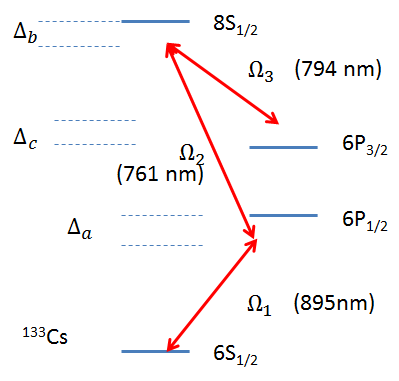
\includegraphics[width=0.5\textwidth]{fig2.png}
    \caption{Cesium atom subjected to three laser fields for nearly resonant excitations}
    \label{fig:sys-2}
\end{figure}

\paragraph{Cesium atom} Consider a simplified cesium level diagram in \prettyref{fig:sys-2} (We ignore Zeeman and hyperfine structure). The laser beams at $895 \mathrm{~nm}, 761 \mathrm{~nm}$ and $794 \mathrm{~nm}$ induce coupling between the ground state $6 \mathrm{~S}_{1 / 2}-6 \mathrm{P}_{1 / 2}$ (with Rabi freq $\left.\Omega_{1}\right), 6 \mathrm{P}_{1 / 2}-8 \mathrm{~S}_{1 / 2}$ (with Rabi freq $\Omega_{2}$ ), and $8 \mathrm{~S}_{1 / 2}-6 \mathrm{P}_{3 / 2}$ (with Rabi freq $\Omega_{3}$ ) respectively. The 1-photon detuning $\Delta_{a}, 2-$ photon detuning $\Delta_{b}$, and 3-photon detuning $\Delta_{c}$ are sketched as in the diagram. We consider the case where all these detunings are at GHz level or smaller, which are tiny comparing with the optical frequencies of the lasers.

Task 1: With $|g\rangle=\left|6 S_{1 / 2}\right\rangle,|a\rangle=\left|6 P_{1 / 2}\right\rangle ;|b\rangle=\left|8 S_{1 / 2}\right\rangle ;|c\rangle=\left|6 P_{3 / 2}\right\rangle$, invent your own additional notations to write down the time-dependent Hamiltonian for the cesium atom in the laser fields, that explicitly have the optical frequencies of the lasers.

Task 2: Write down a time-independent Hamiltonian.

Task 3: Consider radiative life time for $6 P_{1 / 2}, 8 S_{1 / 2}$ and $6 P_{3 / 2}$ are given by $\tau_{a}=$ $1 / \Gamma_{a}, \tau_{b}=1 / \Gamma_{b}$, and $\tau_{c}=1 / \Gamma_{c} .$ Write down the effective non-Hermitian Hamiltonian ${H}_{\mathrm{eff}}$ that includes an anti-Hermitian part to account for the spontaneous emissions.

Task 4: Consider the internal state of the cesium has a wavefunction $\left|\psi_{S}(t)\right\rangle=$ $c_{g}|g\rangle+c_{a}|a\rangle+c_{b}|b\rangle+c_{c}|c\rangle$. Consider the weak perturbation limit (ie laser intensities are small enough that atoms are barely excited), write down the differential equations for the coefficients and approximately solve for $\left|\psi_\text{S}(t)\right\rangle \approx|\tilde{\psi}_\text{S}\rangle$ with $\mathrm{H}_{\mathrm{eff}}|{\tilde{\psi}_{S}}\rangle=0$.

Task 5: Perturbative calculate the 3-photon scattering rate given by $\gamma_{3}=\left|c_{c}\right|^{2} \Gamma$, by assuming $|\psi(t)\rangle$ quickly relax to eigenstate of the effective Hamiltonian with $c_{g} \approx$ $1 .$

Task 6: Consider strong $761 \mathrm{~nm}$ and $795 \mathrm{~nm}$ laser, calculate the atomic polaraizability $\alpha\left(\Omega_{2}, \Omega_{3}\right)$ for the $852 \mathrm{~nm}$ laser excitation by evaluating $\langle\mathrm{d}\rangle=\left\langle\widetilde{\Psi_{S}}\left|d_{a g}\right| a\right\rangle\left\langle g \mid \widetilde{\psi_{S}}\right\rangle+$ c.c., and express it as $\alpha \mathrm{E}_{1}+$ c.c..

Task 7: Discuss the validity of your method of calculating $\gamma_{3}$ and $\alpha\left(\Omega_{2}, \Omega_{3}\right)$ using an ill-defined wavefunction (since its norm cannot be unity) and an effective nonHermitian Hamitonian, instead of using a density matrix and master equations (or the full Monte-Carlo wavefunction method). Your discussion may involve $\Omega, \Delta, \Gamma$ and the total time of observation $\mathrm{T}$.

\paragraph{Solution} \begin{itemize}
\item[(1)] The time-dependent Hamiltonian is 
\begin{equation}
    H = H_0 + H_\text{dipole},
\end{equation}   
where 
\begin{equation}
    H_0 = \hbar \omega_\text{g} \dyad{\text{g}} + \hbar \omega_\text{a} \dyad{\text{a}} 
    + \hbar \omega_\text{b} \dyad{\text{b}} + \hbar \omega_\text{c} \dyad{\text{c}},
\end{equation}
and 
\begin{equation}
    \begin{aligned}
        H_\text{dipole} = &-  \vb*{d}_\text{ag} \cdot (\vb*{E}_1 \ee^{- \ii \omega_1 t} + \vb*{E}_1^* \ee^{\ii \omega_1 t}) \dyad*{\text{a}}{\text{g}} 
        -  \vb*{d}_\text{ba} \cdot (\vb*{E}_2 \ee^{- \ii \omega_2 t} + \vb*{E}_2^* \ee^{ \ii \omega_2 t}) \dyad*{\text{b}}{\text{a}} \\
        & \quad -  \vb*{d}_\text{bc} \cdot (\vb*{E}_3 \ee^{- \ii \omega_3 t } + \vb*{E}_3^* \ee^{ \ii \omega_3 t }) \dyad*{\text{b}}{\text{c}} + \text{h.c.},
    \end{aligned}
\end{equation}
where we denote the external electric fields as 
\begin{equation}
    \vb*{E}_i = \vb*{E}_{i0} \ee^{\ii \omega_i t } + \vb*{E}_{i0}^* \ee^{- \ii \omega_i t}, \quad i = 1, 2, 3.
\end{equation}
The laser frequencies satisfy
\begin{equation}
    \omega_1 + \Delta_\text{a} = \omega_\text{a} - \omega_\text{g}, \quad
    \omega_2 + \Delta_\text{b} - \Delta_\text{a} = \omega_\text{b} - \omega_\text{a}, \quad 
    \omega_3 + \Delta_\text{b} + \Delta_\text{c} = \omega_\text{b} - \omega_\text{c},
\end{equation}
from which we find 
\begin{equation}
    \omega_1 = \omega_\text{a} - \omega_\text{g} - \Delta_\text{a}, \quad 
    \omega_2 = \omega_\text{b} - \omega_\text{a} + \Delta_\text{a} - \Delta_\text{b} , \quad 
    \omega_3 = \omega_\text{b} - \omega_\text{c} - \Delta_\text{b} - \Delta_\text{c}.
\end{equation}
\item[(2)] We switch to the interaction picture, using $H_0$ as the free Hamiltonian, and we have 
\begin{equation}
    \begin{aligned}
        H = H_\text{dipole, int} = &-  \vb*{d}_\text{ag} \cdot (\vb*{E}_1 \ee^{- \ii \omega_1 t} + \vb*{E}_1^* \ee^{\ii \omega_1 t}) \dyad*{\text{a}}{\text{g}} \ee^{\ii (\omega_\text{a} - \omega_\text{g}) t} \\
        &- \vb*{d}_\text{ba} \cdot (\vb*{E}_2 \ee^{- \ii \omega_2 t} + \vb*{E}_2^* \ee^{ \ii \omega_2 t}) \dyad*{\text{b}}{\text{a}} \ee^{\ii (\omega_\text{b} - \omega_\text{a}) t} \\
        & - \vb*{d}_\text{bc} \cdot (\vb*{E}_3 \ee^{- \ii \omega_3 t } + \vb*{E}_3^* \ee^{ \ii \omega_3 t }) \dyad*{\text{b}}{\text{c}} \ee^{\ii (\omega_\text{b} - \omega_\text{c}) t} + \text{h.c.}.
    \end{aligned}
\end{equation}  
We make the rotating wave approximation, i.e. omitting all terms that vibrate much faster than all detunings, 
and get 
\begin{equation}
    \begin{aligned}
        H = & \frac{1}{2} \hbar \Omega_1 \dyad*{\text{a}}{\text{g}} \ee^{\ii (\omega_\text{a} - \omega_\text{g} - \omega_1) t} 
        + \frac{1}{2} \hbar \Omega_2 \dyad*{\text{b}}{\text{a}} \ee^{\ii (\omega_\text{b} - \omega_\text{a} - \omega_2 ) t} \\
        &\quad + \frac{1}{2} \hbar \Omega_3  \dyad*{\text{b}}{\text{c}} \ee^{\ii (\omega_\text{b} - \omega_\text{c} - \omega_3) t} + \text{h.c.},
    \end{aligned}
\end{equation}
where we define 
\begin{equation}
    \frac{1}{2} \hbar \Omega_1 = - \vb*{d}_\text{ag} \cdot \vb*{E}_1, \quad \frac{1}{2} \hbar \Omega_2 = - \vb*{d}_\text{ba} \cdot \vb*{E}_2,
    \quad \frac{1}{2} \hbar \Omega_3 = - \vb*{d}_\text{bc} \cdot \vb*{E}_3.
\end{equation}

\begin{warning*}{}{}
    If we define the electric field as 
    \begin{equation}
        \vb*{E}_i = \frac{1}{2} (\vb*{E}_{i0} \ee^{\ii \omega_i t } + \vb*{E}_{i0}^* \ee^{- \ii \omega_i t}) = \abs*{\vb*{E}_i} \cos(\omega_i t + \varphi_i), \quad i = 1, 2, 3,
        \label{eq:electric-field-alternative}
    \end{equation}
    then there will be no $1/2$ factor in the definition of $\Omega_i$'s. However, later we will evaluate $\expval*{\vb*{d}}$, which has the form of $\text{something} \ee^{- \ii \omega t} + \text{h.c.}$, and if we insist 
    on \eqref{eq:electric-field-alternative}, an additional and easy-to-forget factor $2$ must be added when we 
    evaluate $\alpha = d / E$. 
\end{warning*}

There are three phase factors, and we have four states, so it is possible to use a rotating wave transformation to 
eliminate them all. By  
\begin{equation}
    \begin{aligned}
        &U \ket*{\text{a}} = \ee^{- \ii (\omega_\text{a} - \omega_\text{g} - \omega_1) t} \ket*{\text{a}} = \ee^{ - \ii \Delta_\text{a} t} \ket*{\text{a}}  , \\
        &U \ket*{\text{b}} = \ee^{- \ii (\omega_\text{b} - \omega_\text{a} - \omega_2 ) t} \ee^{ - \ii \Delta_\text{a} t}  \ket*{\text{b}} = \ee^{- \ii \Delta_\text{b} t} \ket*{\text{b}}, \\
        &U \ket*{\text{c}} = \ee^{- \ii (\omega_\text{b} - \omega_\text{c} - \omega_3) t} \ee^{ \ii \Delta_\text{b} t} \ket*{\text{c}} = \ee^{\ii \Delta_\text{c} t},
    \end{aligned}
\end{equation}
we have 
\begin{equation}
    \begin{aligned}
        H \to H' &= U H U^\dagger - \ii \hbar U \partial_t U^\dagger \\
        &= \frac{1}{2} \hbar \Omega_1 \dyad*{\text{a}}{\text{g}} + \frac{1}{2} \hbar \Omega_2 \dyad*{\text{b}}{\text{a}} + \frac{1}{2} \hbar \Omega_3  \dyad*{\text{b}}{\text{c}} + \text{h.c.} + \hbar \Delta_\text{a} \dyad*{\text{a}} + \hbar \Delta_\text{b} \dyad{\text{b}} - \hbar \Delta_\text{c} \dyad{\text{c}}.
    \end{aligned}
\end{equation}
This is the time-independent Hamiltonian we want.
\item[(3)] The effective Hamiltonian is 
\begin{equation}
    \begin{aligned}
        H_\text{eff}& = \frac{1}{2} \hbar \Omega_1 \dyad*{\text{a}}{\text{g}} + \frac{1}{2} \hbar \Omega_2 \dyad*{\text{b}}{\text{a}} + \frac{1}{2} \hbar \Omega_3  \dyad*{\text{b}}{\text{c}} + \text{h.c.} + \hbar \underbrace{\left( \Delta_\text{a} - \frac{\ii \Gamma_\text{a}}{2} \right)}_{\tilde{\Delta}_\text{a}} \dyad*{\text{a}} \\
        &\quad + \hbar \underbrace{\left( \Delta_\text{b} - \frac{\ii \Gamma_\text{b}}{2} \right)}_{\tilde{\Delta}_\text{b}} \dyad{\text{b}} - \hbar \underbrace{\left( \Delta_\text{c} + \frac{\ii \Gamma_\text{c}}{2} \right)}_{\tilde{\Delta}_\text{c}} \dyad{\text{c}} .
    \end{aligned}
\end{equation} 

\item[(4)] In the weak perturbation limit, $c_\text{g} \approx 1$, and the equation 
$H_\text{eff} \ket*{\psi_\text{s}} = 0$ is equivalent to 
\[
    \begin{aligned}
        &- \frac{1}{2} \hbar \Omega_1^* c_\text{a} = 0, \\
        & \frac{1}{2} \hbar \Omega_1 + \hbar \left( \Delta_\text{a} - \frac{\ii \Gamma_\text{a}}{2}  \right) c_\text{a} + \frac{1}{2} \hbar \Omega_2^* c_\text{b} = 0, \\
        &\frac{1}{2} \hbar \Omega_2 c_\text{a} + \hbar \left( \Delta_\text{b} - \frac{\ii \Gamma_\text{b}}{2}  \right) c_\text{b} + \frac{1}{2} \hbar \Omega_3 c_\text{c} = 0, \\
        &\frac{1}{2} \hbar \Omega_3^* - \hbar \left( \Delta_\text{c} + \frac{\ii \Gamma_\text{c}}{2} \right) c_\text{c} = 0.
    \end{aligned}
\]
The first equation can be throw away because it merely means $c_\text{a}$ is small. The solutions are therefore 
\begin{equation}
    \begin{aligned}
        c_\text{a} &= - \frac{2 \Omega_1 \tilde{\Delta}_\text{b} \tilde{\Delta}_\text{c} +  \abs*{\Omega_3}^2 \Omega_1 / 2 }{ \abs*{\Omega_3}^2 \tilde{\Delta}_\text{a} + 4 \tilde{\Delta}_\text{a} \tilde{\Delta}_\text{b} \tilde{\Delta}_\text{c} - \abs*{\Omega_2}^2 \tilde{\Delta}_\text{c} }, \\
        c_\text{b} &= \frac{\Omega_1 \Omega_2 \tilde{\Delta}_\text{c}}{ \abs*{\Omega_3}^2 \tilde{\Delta}_\text{a} + 4 \tilde{\Delta}_\text{a} \tilde{\Delta}_\text{b} \tilde{\Delta}_\text{c} - \abs*{\Omega_2}^2 \tilde{\Delta}_\text{c} }, \\
        c_\text{c} &= \frac{\Omega_1 \Omega_2 \Omega_3^* / 2 }{ \abs*{\Omega_3}^2 \tilde{\Delta}_\text{a} + 4 \tilde{\Delta}_\text{a} \tilde{\Delta}_\text{b} \tilde{\Delta}_\text{c} - \abs*{\Omega_2}^2 \tilde{\Delta}_\text{c} }.
    \end{aligned}
    \label{eq:perturbation-results-2}
\end{equation}

\begin{note*}{}
    What we are doing here is equivalent to the first order perturbation theory, i.e. giving the eigenstate a 
    first order correction withing correcting the energy. We are assuming that $H_\text{eff} \ket*{\text{ground}} = 0$
    because before perturbation, the energy of the ground state is zero. If it is not, we need to change the 
    RHS of the equation. This is often called \concept{adiabatic elimination}. See the discussion below  
    \eqref{next-eq:gamma-2-1} \href{../5/5-discussion.pdf}{here}.
\end{note*}

\item[(5)] We have 
\begin{equation}
    \gamma_3 = \Gamma_3 \abs*{c_\text{c}}^2 = \frac{\abs*{\Omega_1}^2 \abs*{\Omega_2}^2 \abs*{\Omega_3}^2 / 4 }{ \abs*{\abs*{\Omega_3}^2 \tilde{\Delta}_\text{a} + 4 \tilde{\Delta}_\text{a} \tilde{\Delta}_\text{b} \tilde{\Delta}_\text{c} - \abs*{\Omega_2}^2 \tilde{\Delta}_\text{c}}^2 } \Gamma_3.
\end{equation} 

\item[(6)] The total unitary transformation from the original picture to the current pictures is partly given by 
\[
    U_\text{total} \ket*{\text{g}} = \ee^{\ii \omega_\text{g} t} \ket*{\text{g}}, \quad 
    U_\text{total} \ket*{\text{a}} = \ee^{- \ii (\omega_\text{a} - \omega_\text{g} - \omega_1) t} \ee^{\ii \omega_\text{a} t} \ket*{\text{a}} , 
\]
so in the current picture, we have 
\[
    \vb*{d} = U_\text{total} \vb*{d}_\text{original} U_\text{total}^{-1}, 
\]
and therefore 
\begin{equation}
    \begin{aligned}
        \expval*{\vb*{d}} &= \braket*{\psi_\text{s}}{\text{a}} \ee^{\ii (\omega_1 + \omega_\text{g}) t} \vb*{d}_\text{ag} \ee^{- \ii \omega_\text{g} t} \braket*{\text{g}}{\psi_\text{s}} + \text{h.c.} = \ee^{- \ii \omega_1 t} \vb*{d}_\text{ga} \braket*{\psi_\text{s}}{\text{g}} \braket*{\text{a}}{\psi_\text{s}} + \text{h.c.} \\
        &= - \ee^{- \ii \omega_1 t} \vb*{d}_\text{ga} \frac{-2 \vb*{d}_\text{ag} \cdot \vb*{E}_1}{\hbar} \frac{2 \tilde{\Delta}_\text{b} \tilde{\Delta}_\text{c} +  \abs*{\Omega_3}^2  / 2 }{ \abs*{\Omega_3}^2 \tilde{\Delta}_\text{a} + 4 \tilde{\Delta}_\text{a} \tilde{\Delta}_\text{b} \tilde{\Delta}_\text{c} - \abs*{\Omega_2}^2 \tilde{\Delta}_\text{c} } + \text{h.c.}  ,
    \end{aligned}
\end{equation}
so we have 
\begin{equation}
    \tensor{\vb*{\alpha}} = \frac{ \vb*{d}_\text{ga} \vb*{d}_\text{ag}}{\hbar} \frac{4 \tilde{\Delta}_\text{b} \tilde{\Delta}_\text{c} +  \abs*{\Omega_3}^2 }{ \abs*{\Omega_3}^2 \tilde{\Delta}_\text{a} + 4 \tilde{\Delta}_\text{a} \tilde{\Delta}_\text{b} \tilde{\Delta}_\text{c} - \abs*{\Omega_2}^2 \tilde{\Delta}_\text{c} } .
\end{equation}
When the other two laser beams are very, very strong, we have approximately 
\begin{equation}
    \tensor{\vb*{\alpha}} = \frac{ \vb*{d}_\text{ga} \vb*{d}_\text{ag}}{\hbar} \frac{ \abs*{\Omega_3}^2 }{ \abs*{\Omega_3}^2 \tilde{\Delta}_\text{a} - \abs*{\Omega_2}^2 \tilde{\Delta}_\text{c} } .
\end{equation}

\item[(7)] What we are doing is to assume (a) that quantum jump is highly impossible on the time scale that we 
are interested, so the main effect of spontaneous radiation is to renormalize parameters in a pure state problem,
and (b) that all perturbations, be it from $\Omega$ or $\Gamma$, are small enough. 

The first condition is equivalent to $\gamma T \ll 1$, where $T$ is the time scale we are interested in, where 
\begin{equation}
    \Gamma \sim \Gamma_\text{a} \abs*{c_\text{a}}^2 + \Gamma_\text{b} \abs*{c_\text{b}}^2 + \Gamma_\text{c} \abs*{c_\text{c}}^2.
\end{equation}
The second condition is equivalent to $\abs*{c_\text{a}}^2 + \abs*{c_\text{b}}^2 + \abs*{c_\text{c}}^2 \ll 1$. 

\end{itemize}

\begin{figure}
    \centering
    

\tikzset{every picture/.style={line width=0.75pt}} %set default line width to 0.75pt        

\begin{tikzpicture}[x=0.75pt,y=0.75pt,yscale=-1,xscale=1]
%uncomment if require: \path (0,300); %set diagram left start at 0, and has height of 300

%Straight Lines [id:da3132242130750498] 
\draw    (84,137) -- (130,137) ;
%Straight Lines [id:da8852176090904664] 
\draw    (232,119) -- (278,119) ;
%Straight Lines [id:da3118336041065983] 
\draw    (142,51) -- (188,51) ;
%Straight Lines [id:da13043475932345627] 
\draw    (144,224) -- (190,224) ;
%Straight Lines [id:da1403435354778697] 
\draw    (165,51) -- (108.12,135.34) ;
\draw [shift={(107,137)}, rotate = 304] [fill={rgb, 255:red, 0; green, 0; blue, 0 }  ][line width=0.08]  [draw opacity=0] (12,-3) -- (0,0) -- (12,3) -- cycle    ;
%Straight Lines [id:da048714045175360265] 
\draw    (165,51) -- (253.4,117.79) ;
\draw [shift={(255,119)}, rotate = 217.07] [fill={rgb, 255:red, 0; green, 0; blue, 0 }  ][line width=0.08]  [draw opacity=0] (12,-3) -- (0,0) -- (12,3) -- cycle    ;
%Straight Lines [id:da3087053085673217] 
\draw    (107,137) -- (165.86,222.35) ;
\draw [shift={(167,224)}, rotate = 235.41] [fill={rgb, 255:red, 0; green, 0; blue, 0 }  ][line width=0.08]  [draw opacity=0] (12,-3) -- (0,0) -- (12,3) -- cycle    ;
%Straight Lines [id:da2241090509364947] 
\draw    (255,119) -- (168.28,222.47) ;
\draw [shift={(167,224)}, rotate = 309.97] [fill={rgb, 255:red, 0; green, 0; blue, 0 }  ][line width=0.08]  [draw opacity=0] (12,-3) -- (0,0) -- (12,3) -- cycle    ;

% Text Node
\draw (280,119) node [anchor=west] [inner sep=0.75pt]   [align=left] {c};
% Text Node
\draw (82,137) node [anchor=east] [inner sep=0.75pt]   [align=left] {a};
% Text Node
\draw (142,224) node [anchor=east] [inner sep=0.75pt]   [align=left] {g};
% Text Node
\draw (140,51) node [anchor=east] [inner sep=0.75pt]   [align=left] {b};


\end{tikzpicture}

    \caption{The energy level diagram of the diamond system that looks more like a diamond}
    \label{fig:diamond}
\end{figure}

\paragraph{Discussion} What we are doing in this problem is actually exactly solving a non-perturbative 
optical problem with perturbative techniques. When the external driving field is not that strong and the 
detuning is large, we can safely use perturbation theory. When the external driving field is very strong 
(so that electrons can be pulled out of an atom and then squeezed back), or the detuning is small, 
purely perturbative calculation does not work. 

Now we go back to the problem. The energy level diagram that shows how spontaneous radiation happens is 
\prettyref{fig:diamond}. Note that it is impossible to jump from $\ket*{\text{a}}$ to $\ket*{\text{g}}$,
because if spontaneous radiation channels in \prettyref{fig:diamond} are possible, then $\ket*{\text{b}}$
and $\ket*{\text{g}}$ have the same parity, $\ket*{\text{a}}$ and $\ket*{\text{c}}$ have the same parity, 
and $\ket*{\text{b}}$ and $\ket*{\text{a}}$ have opposite parities. 
Therefore, there is no single-photon process from $\ket*{\text{b}}$ to $\ket*{\text{g}}$.
Since we are not interested in where the atom ends in, the quantum jump operators are thrown away,
and we just study $H_\text{eff}$.

Now we go on to discuss when the perturbative calculation in Task 4 works. We can expect the atom is largely on 
the ground state only when $\vb*{E}_1$ is small and has a relatively large detuning. This imposes \emph{no} 
constraints on $\vb*{E}_2$ and $\vb*{E}_3$. Therefore, as long as the conditions about $\vb*{E}_1$ are 
correct, and RWA works, the perturbative calculation in Task 4 works. Our calculation is therefore 
perturbative for $\vb*{E}_1$ but \emph{non} perturbative for $\vb*{E}_2$ and $\vb*{E}_3$. This fact can also 
be seen from \eqref{eq:perturbation-results-2}, where everything is proportion to $\Omega_1 \propto \vb*{E}_1$.

Finally, we can see from \prettyref{fig:sys-2} that what we are actually dealing with is a three-photon 
process that carries the atom from $\ket*{\text{g}}$ to $\ket*{\text{c}}$. This can also be seen from 
$c_\text{c}$ in \eqref{eq:perturbation-results-2}. If carrying the atom to $\ket*{\text{c}}$ is all what 
we care, and we are not interested by the detailed dynamics, then the condition in Task 7 can be loosen, 
because even though quantum jumps occur from time to time, the atom quickly relaxes to $\ket*{\psi_\text{s}}$
after one quantum jump. The atom is therefore almost constantly at $\ket*{\psi_\text{s}}$.
In perturbative calculation of nonlinear effects, we sum up several diagrams like \prettyref{fig:sys-2}, but 
the Hamiltonian has not undergone RWA. What we are doing here is actually a resummation of these ``bare'' diagrams
into one diagram \prettyref{fig:sys-2}, and then diagonalize it.

\paragraph{}

\begin{figure}
    \centering
    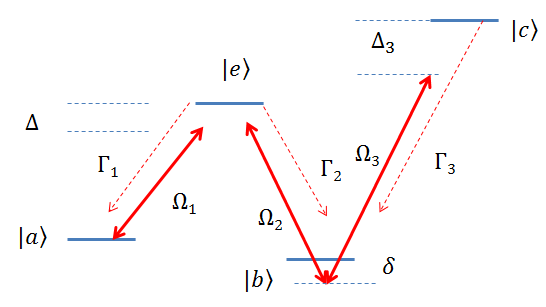
\includegraphics[width=0.7\textwidth]{fig3.png}
    \caption{A three-level system coupled to an additional energy level}
    \label{fig:sys-3}
\end{figure}

\paragraph{EIT-assisted giant Kerr effect} The ``lambda''-system composed of $|\text{a}\rangle,|\text{e}\rangle,|\text{b}\rangle$ is further coupled to excited state $|\text{c}\rangle$, as in \prettyref{fig:sys-3}. We consider the situation of EIT-resonance: $\delta=0$. We further consider atomic state to be initially in $|\psi(t=0)\rangle=|\mathrm{a}\rangle$, and weak-excitation limit is satisfied $\left(\left|\Omega_{1}\right|\right.$ small "enough").
(a) Write down the effective Hamiltonian for this problem for $\delta=0$.
(b) Obtain the approximate stochastic wavefunction in its steady state $|\tilde{\psi}_\text{S}\rangle=|\text{a}\rangle+$ ${c}_{\mathrm{e}}|\text{e}\rangle+c_\text{b}|\text{b}\rangle+c_\text{c}|\text{c}\rangle$ such that ${H}_{\mathrm{eff}}\left|\psi_{\mathrm{S}}\right\rangle \approx 0$.
(c) Approximately evaluate the atomic dipole moment $\langle {d}\rangle=\left\langle\psi_{S}\left|d_{a e}\right| a\right\rangle\left\langle e \mid \psi_{S}\right\rangle+$ c.c. oscillating at the $\mathrm{E}_{1}$ frequency.

\paragraph{Solution} \begin{itemize}
\item[(a)] Repeating procedures in Task 1 of the previous problem, after RWA, we have 
\begin{equation}
    H = H_0 + \frac{1}{2} \hbar \Omega_1 \dyad*{\text{e}}{\text{a}} \ee^{- \ii \omega_1 t} 
    + \frac{1}{2} \hbar \Omega_2 \dyad*{\text{e}}{\text{b}} \ee^{- \ii \omega_2 t} 
    + \frac{1}{2} \hbar \Omega_3 \dyad*{\text{c}}{\text{b}} \ee^{- \ii \omega_3 t} + \text{h.c.},
\end{equation}  
where 
\begin{equation}
    H_0 = \hbar \omega_\text{a} \dyad*{\text{a}} + \hbar \omega_\text{e} \dyad*{\text{e}}
    + \hbar \omega_\text{b} \dyad*{\text{b}} + \hbar \omega_\text{c} \dyad*{\text{c}}.
\end{equation}
Switching to the interaction picture, the Hamiltonian becomes 
\begin{equation}
    H = \frac{1}{2} \hbar \Omega_1 \dyad*{\text{e}}{\text{a}} \ee^{ \ii ( \omega_\text{e} - \omega_\text{a} - \omega_1 ) t} 
    + \frac{1}{2} \hbar \Omega_2 \dyad*{\text{e}}{\text{b}} \ee^{ \ii (\omega_\text{e} - \omega_\text{b} - \omega_2 ) t} 
    + \frac{1}{2} \hbar \Omega_3 \dyad*{\text{c}}{\text{b}} \ee^{\ii ( \omega_\text{c} - \omega_\text{b} - \omega_3) t} + \text{h.c.}.
    \label{eq:ham-int-origin}
\end{equation}
The detunings are 
\begin{equation}
    \Delta + \omega_1 = \omega_\text{e} - \omega_\text{a}, \quad 
    \omega_\text{e} - \omega_\text{b} = \omega_2, \quad
    \Delta_3 + \omega_3 = \omega_\text{c} - \omega_\text{b},
\end{equation}
so \eqref{eq:electric-field-alternative} is 
\begin{equation}
    H = \frac{1}{2} \hbar \Omega_1 \dyad*{\text{e}}{\text{a}} \ee^{\ii \Delta t} 
    + \frac{1}{2} \hbar \Omega_2 \dyad*{\text{e}}{\text{b}} 
    + \frac{1}{2} \hbar \Omega_3 \dyad*{\text{c}}{\text{b}} \ee^{\ii \Delta_3 t} + \text{h.c.}.
\end{equation} 
Now we do rotating wave transformation 
\begin{equation}
    U \ket*{\text{e}} = \ee^{- \ii \Delta t} \ket*{\text{e}}, \quad 
    U \ket*{\text{c}} = \ee^{- \ii \Delta_3 t} \ket*{\text{c}}, \quad 
    U \ket*{\text{a}} = \ket*{\text{a}}, \quad U \ket*{\text{b}} = \ket*{\text{b}},
\end{equation}
we have 
\begin{equation}
    \begin{aligned}
        H \to H' &= U H U^\dagger - \ii \hbar U \partial_t U^\dagger \\
        &= \frac{1}{2} \hbar \Omega_1 \dyad*{\text{e}}{\text{a}} \ee^{\ii \Delta t} 
        + \frac{1}{2} \hbar \Omega_2 \dyad*{\text{e}}{\text{b}} 
        + \frac{1}{2} \hbar \Omega_3 \dyad*{\text{c}}{\text{b}} \ee^{\ii \Delta_3 t} + \text{h.c.}
        + \hbar \Delta \dyad{\text{e}} + \hbar \Delta_3 \dyad*{\text{c}}.
    \end{aligned}
    \label{eq:ham-3}
\end{equation}
The effective Hamiltonian can be obtained by adding the damping terms, i.e. 
\begin{equation}
    \begin{aligned}
        H_\text{eff} &= \frac{1}{2} \hbar \Omega_1 \dyad*{\text{e}}{\text{a}} \ee^{\ii \Delta t} 
        + \frac{1}{2} \hbar \Omega_2 \dyad*{\text{e}}{\text{b}} 
        + \frac{1}{2} \hbar \Omega_3 \dyad*{\text{c}}{\text{b}} \ee^{\ii \Delta_3 t} + \text{h.c.} \\
        &\quad + \hbar \Delta \dyad{\text{e}} + \hbar \Delta_3 \dyad*{\text{c}}
        - \frac{\ii \hbar (\Gamma_1 + \Gamma_2)}{2} \dyad{\text{e}} - \frac{\ii \hbar \Gamma_3}{2} \dyad*{\text{c}}.
    \end{aligned}
\end{equation}

\item[(b)] The equation $H_\text{eff} \ket*{\tilde{\psi}_\text{s}} \approx 0$ is equivalent to 
\[
    \begin{aligned}
        & \frac{1}{2} \hbar \Omega_1^* c_\text{e} = 0, \\
        & \frac{1}{2} \hbar \Omega_1 + \frac{1}{2} \hbar \Omega_2 c_\text{b} + \hbar \left( \Delta - \frac{\ii (\Gamma_1 + \Gamma_2)}{2} \right) c_\text{e} = 0, \\
        & \frac{1}{2} \hbar \Omega_2^* c_\text{e} + \frac{1}{2} \hbar \Omega_3^* c_\text{c} = 0, \\
        & \frac{1}{2} \hbar \Omega_3 c_\text{b} + \hbar \left( \Delta_3 - \frac{\ii \Gamma_3}{2} \right) c_\text{c} = 0.
    \end{aligned}
\] 
We throw away the first equation because it merely requires that $c_\text{c}$ is small, and solving the rest 
of the equations gives 
\begin{equation}
    \begin{aligned}
        c_\text{b} &= - \frac{\Omega_1 \Omega_2^* \tilde{\Delta}_3 }{ \abs*{\Omega_2}^2 \tilde{\Delta}_3 + \abs*{\Omega_3}^2 \tilde{\Delta}}, \\
        c_\text{c} &= \frac{\Omega_1 \Omega_2^* \Omega_3}{2 (\abs*{\Omega_2}^2 \tilde{\Delta}_3 + \abs*{\Omega_3}^2 \tilde{\Delta}) } , \\
        c_\text{e} &= - \frac{\Omega_1 \abs*{\Omega_3}^2}{2 (\abs*{\Omega_2}^2 \tilde{\Delta}_3 + \abs*{\Omega_3}^2 \tilde{\Delta}) },
    \end{aligned}
\end{equation}
where we define 
\begin{equation}
    \tilde{\Delta} = \Delta - \frac{\ii (\Gamma_1 + \Gamma_2)}{2}, \quad \tilde{\Delta}_3 = \Delta_3 - \frac{\ii \Gamma_3}{2}.
\end{equation}

\item[(c)] The total picture transformation from the original picture to the picture we are using is 
\begin{equation}
    U_\text{total} \ket*{\text{a}} = \ee^{\ii \omega_\text{a} t} \ket*{\text{a}}, \quad 
    U_\text{total} \ket*{\text{e}} = \ee^{- \ii \Delta t} \ee^{\ii \omega_\text{e} t} \ket*{\text{e}} = \ee^{\ii (\omega_1 + \omega_\text{a}) t} ,
\end{equation} 
and therefore in the current picture, we have 
\[
    \mel{\text{e}}{\vb*{d}}{\text{a}} = \mel{\text{e}}{U_\text{total} \vb*{d}_\text{original} U_\text{total}^\dagger }{\text{a}} = \vb*{d}_\text{ea} \ee^{\ii \omega_1 t}, \quad \mel{\text{a}}{\vb*{d}}{\text{e}} = \vb*{d}_\text{ae}  \ee^{- \ii \omega_1 t},
\]
so
\begin{equation}
    \begin{aligned}
        \expval*{\vb*{d}} &= \vb*{d}_\text{ae} \ee^{- \ii \omega_1 t} \braket*{\psi_\text{s}}{\text{a}} \braket*{\text{e}}{\psi_\text{s}} + \text{h.c.} \\
        &= \frac{\vb*{d}_\text{ae} \vb*{d}_\text{ea} \cdot \vb*{E}_{10} \ee^{- \ii \omega_1 t} }{\hbar} 
        \frac{\abs*{\Omega_3}^2}{\abs*{\Omega_2}^2 \tilde{\Delta}_3 + \abs*{\Omega_3}^2 \tilde{\Delta}} + \text{h.c.}.
    \end{aligned}
\end{equation}

\end{itemize}

\paragraph{Discussion} Kerr effect means the fact that the one beam of light can affect the refractive index 
of another beam of light. The system is said to be \emph{giant} because it can be extremely sensible.
% TODO

Unfortunately, the system \prettyref{fig:sys-3} has been proven impossible to be implemented in a random gas.
It is possible to be implemented in a ultracold atom system, but optics in strongly correlated systems is still
a big problem. 

The random wave function + perturbation theory approach used in this problem is already dangerous, because when 
$\Omega_2$ is small, it is possible that the meta-stable state has a large $\ket*{\text{b}}$ component.

\paragraph{}

\begin{figure}
    \centering
    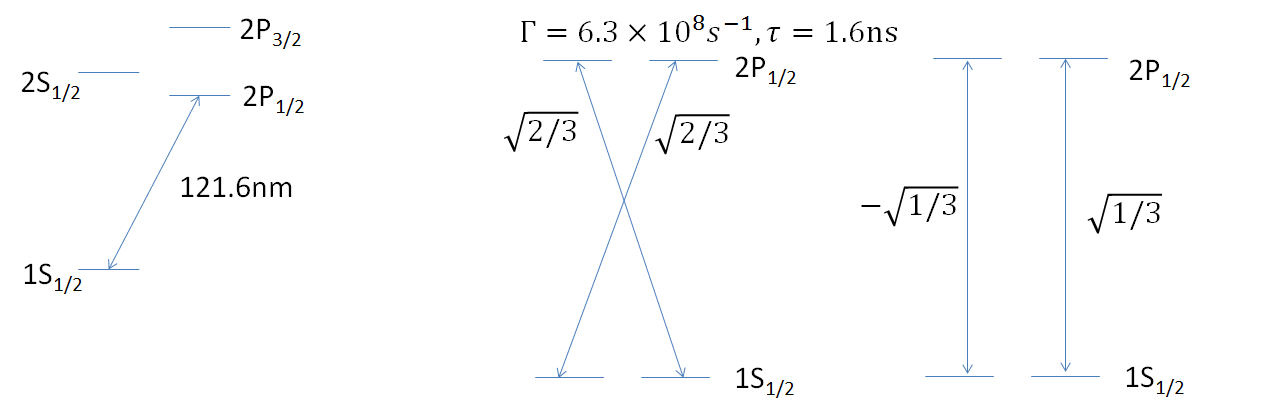
\includegraphics[width=0.8\textwidth]{fig4.png}
    \caption{Left: Simplified Hydrogen levels and excitation of $1 \mathrm{~S}$ atom with $121.6 \mathrm{~nm}$ light resonant to $1 \mathrm{~S}-2 \mathrm{P}_{1 / 2}$ transition. Right: The Clebsch-Gordon coefficients for the $1 \mathrm{~S}_{1 / 2}-2 \mathrm{P}_{1 / 2}$ dipole transitions.}
    \label{fig:sys-4}
\end{figure}

\paragraph{Effective Hamiltonian and Master Equation for the Hydrogen ``D1'' manifold} 
This problem exercises on setting up effective Hamiltonian and master equation for multi-level system including radiative decays. We choose hydrogen atom as an example, and for simplicity we ignore the hyperfine structure.

We consider a hydrogen atom subjected to $121.6 \mathrm{~nm}$ laser radiation. The laser is linearly polarized, and its frequency is exactly resonant to the $2 \mathrm{~S}_{1 / 2}-2 \mathrm{P}_{1 / 2}$ transition. The Rabi frequency is defined as $\Omega=\frac{E\left\langle 1 S_{1 / 2}, m\left|d_{z}\right| 2 P_{1 / 2}, m\right\rangle}{\hbar}$, and we choose the polarization direction of light to be along $z$, which is also chosen to be the quantization axis.

(a) Write down the non-Hermitian effective Hamiltonian matrix that includes both light-atom interaction and the radiative decay from $2 \mathrm{P}_{1 / 2}$, in the rotating frame with no explicit time-dependence.
(b) Write down the Master equation for the density matrix.

\paragraph{Solution} \begin{itemize}
\item[(a)] After coupling the orbital angular momentum and the spin angular momentum together, for $\text{S}$
we get $j=1/2, m_j = \pm 1/2$, and for $\text{P}$ we have $j = 1/2, m_j = \pm 1/2$, and 
$j = 3/2, m_j = \pm 1/2, \pm 3/2$. These are shown in \prettyref{fig:sys-4}, and the external laser connects
$1 \text{S}_{1/2}$ and $2 \text{P}_{1/2}$. Since the direction of $\vb*{E}$ is $z$ direction, the atom-light 
coupling Hamiltonian is proportion to $z$, and since $\comm*{z}{L_z} = 0$, and spins are not directly coupled 
to $\vb*{E}$, we find $J_z = L_z + S_z$ is conserved. Therefore, there are four 
states that are involved in the presence of the \SI{121.6}{nm} laser radiation: $1 \text{S}_{1/2}, m = \pm 1/2$, 
$2 \text{P}_{1/2}, m = \pm 1/2$, and only states with the same $m$ can be coupled. 

To be concise we consider $1 \text{S}_{1/2}$ to be $\text{g}$ and $2 \text{P}_{1/2}$ to be $\text{e}$.
So the Hamiltonian after RWA is 
\begin{equation}
    H = - \sum_{m = \pm 1/2} \hbar \Omega_{m} \dyad*{\text{e}, m}{\text{g}, m} \ee^{\ii (\omega_\text{e} - \omega_\text{g} - \omega)} + \text{h.c.}.
\end{equation}
Since the detuning 
\begin{equation}
    \Delta = \omega_\text{e} - \omega_\text{g} - \omega
\end{equation}
is zero, the RWA Hamiltonian is 
\begin{equation}
    H = - \sum_{m = \pm 1/2} \hbar \Omega_m \dyad*{\text{e}, m}{\text{g}, m} + \text{h.c.}.
\end{equation}

Now we include the damping terms. Note that the polarization of spontaneous radiation is not necessarily 
along the $z$ axis. Emission of a $\sigma_+$ photon introduces a $1/2 \to -1/2$ decay channel. Emission of 
a $\sigma_-$ photon introduces a $-1/2 \to 1/2$ decay channel. Emission of a $\pi$ photon introduces
$1/2 \to 1/2$, $-1/2 \to -1/2$ channels. Therefore 
\begin{equation}
    \begin{aligned}
        &C_{\sigma_+} = \sqrt{\frac{2}{3} \Gamma_\text{ge}} \dyad*{\text{g}, -1/2}{\text{e}, 1/2} , \quad 
        C_{\sigma_-} = \sqrt{\frac{2}{3} \Gamma_\text{ge}} \dyad*{\text{g}, 1/2}{\text{e}, -1/2} , \\
        &C_{\pi} = - \sqrt{\frac{1}{3} \Gamma_\text{ge}} \dyad*{\text{g}, -1/2}{\text{e}, -1/2}
        + \sqrt{\frac{1}{3} \Gamma_\text{ge}} \dyad*{\text{g}, 1/2}{\text{e}, 1/2},
    \end{aligned}
\end{equation}
and 
\begin{equation}
    \begin{aligned}
        H_\text{eff} &= - \sum_{m = \pm 1/2} \hbar \Omega_m \dyad*{\text{e}, m}{\text{g}, m} + \text{h.c.} - \frac{\ii \hbar}{2} \sum_{p = \sigma_+, \sigma_-, \pi} C^\dagger_p C_p \\
        &= - \hbar \Omega_m (\dyad*{\text{e}, 1/2}{\text{g}, 1/2} - \dyad*{\text{e}, -1/2}{\text{g}, -1/2}) + \text{h.c.} \\
        &\quad - \frac{\ii \hbar}{2} \Gamma_\text{ge} (\dyad{\text{e}, -1/2} + \dyad{\text{e}, 1/2}).
    \end{aligned}
\end{equation}

\begin{warning*}{}{}
    Note that the Wigner–Eckart theorem 
    \begin{equation}
        \langle j\,m|T_{q}^{(k)}|j'\,m'\rangle =\langle j'\,m'\,k\,q|j\,m\rangle \langle j\|T^{(k)}\|j'\rangle
    \end{equation}
    tells us that the dipole Hamiltonian is proportion to C-G coefficients, and therefore $\Omega_+ = - \Omega_-$.
\end{warning*}

\item[(b)] The master equation is just 
\begin{equation}
    \dot{\rho} = \frac{1}{\ii \hbar} ( H_\text{eff} \rho - \rho H_\text{eff}^\dagger ) + \sum_{p = \sigma_+, \sigma_-, \pi} C^\dagger_p \rho C_p.
\end{equation}

\begin{note*}{}{}
    Note that in a time evolution equation according to a non-Hermitian effective Hamiltonian, we should
    \emph{not} use the commutator.
\end{note*}

\end{itemize}

\end{document}